\chapter{Literature review}

\section*{Introduction}
\subsection*{Methodology}
The approach adopted in this literature review is intermediate between a systematic approach and a survey of related works.
The justification for this singular approach is that many domains are presented, some containing several tens of thousands of articles.
For this reason, a systematic approach would be too cumbersome, while a survey would not reflect the richness of each field.

First, the scope of the literature review will be defined through research hypotheses.
Once these hypotheses are created, queries will be made on a bibliographic database.
The queries will be performed on Scopus~\footnote{https://www.scopus.com/}, which offers a larger number of references than the Web of Science and more tools for query design.

The results obtained will then be analyzed from several angles. First of all, the evolution of the volume of publications returned by the query, to attempt to represent the interest in the topic.
Secondly, an analysis of the keywords will be made through VOSviewer~\footnote{https://www.vosviewer.com/} "a software tool for constructing and visualizing bibliometric networks".
Especially VOSviewer allows to visualize bibliographic features such as the network of authors or of keywords.
The keywords used by the different articles fetched by the request provide valuable insights on the evolution of a given field, especially on its interdisciplinary aspect.
Finally, a review of some of the most influential articles from the query result will be discussed.
The influence criteria will be the number of citations.
%TODO Explain the exclusion of the conference tracks presentation and reviews papers in all the request.

This methodology aims to provide a sufficient understanding of the interest and evolution of the topics explored, as well as answers related to the subproblematics exposed.

\subsection*{Hypotheses}
This manuscript is limited in the scientific domain investigated.
Thus, the following working hypotheses will delimit the work presented.

\begin{itemize}
    \item 1. On social media data: social media data have a low ratio information/noise and are as trustworthy as phone calls. Clean, well-written textual data are then excluded.
    \item 2. On crisis management: the crisis management context is particular and this manuscript focuses on the response phase and its context.
    \item 3. On improving the decision making process: improving decision making means improving situational awareness and coordination among the various actors.
\end{itemize}

Having these hypotheses, the literature review presented in this chapter explores the context around the different problematics raised in the previous chapter.
As a reminder, the main problem of this manuscript is: \emph{How to design an information system able to automatically manage and deliver relevant information extracted from social media data during crisis response?}
This main problematic is decomposed among three sub problematics:

\begin{itemize}
    \item What information that can be obtained from social media is relevant to the decisiom makers in crisis response?
    \item How can these information be obtained, in the context of crisis informatic?
    \item How are these information organised to deliver the value expected by decision makers?
\end{itemize}

The first section of this chapter presents the work related to the main problematic and specially systems developped to automatically process social media during crisis response.
Then, the second section explores the first sub problematic and the different representations of information used by previous work.
Finally, the third section overlook social media processing by NLP in general to provide context for the second sub problematic.
As the last sub problematic is similar to the one of the main problematic, its literature review will be merge into the first section.

\section{Information systems for crisis response fed with social media data}
Chapter 1 identified the opportunities offered by social media to support crisis response.
Many researchers explored that opportunities and built systems and architecture to mine data and provide their insights to decision makers.
This first part of the literature review intends to highlight the systems built for this purpose.
The question that this parts aims to answer is: \emph{What are the existing social media processing system developped for crisis response over the years?}

To answer this question, the following request was made on the Scopus database.

\begin{itemize}
    \item SUBJAREA(comp)
    \item AND (TITLE-ABS-KEY({crisis management} or {crisis response} or contingency or {disaster response} or {disaster management}))
    \item AND (TITLE-ABS-KEY ({social media} or twitter))
    \item AND (TITLE-ABS-KEY(system and processing))
    \item AND ( EXCLUDE ( DOCTYPE,"re" ) OR EXCLUDE ( DOCTYPE,"cr" ) )
\end{itemize}

The request returns papers that:

\begin{itemize}
    \item Are in the computer science domain, as this domain contains both the AI and Information Systems domains.
    \item Are centered around crises|disasters management|response or contingency plans.
    \item That present systems that process data
    \item Papers that present conference tracks and reviews are excluded.
\end{itemize}

The request returns 96 documents, published between 2011 and 2021.
The beginning of this domain of research corresponds to the democratization of social media, with the development of social media plaforms happening during the 2000-2010 period (Figure~\ref{literature:crisis-informatic-hist}).
Naturally, the field has developed, driven by the need of crisis management organizations and the public interest benefit it promises.

\begin{figure}[htb]
    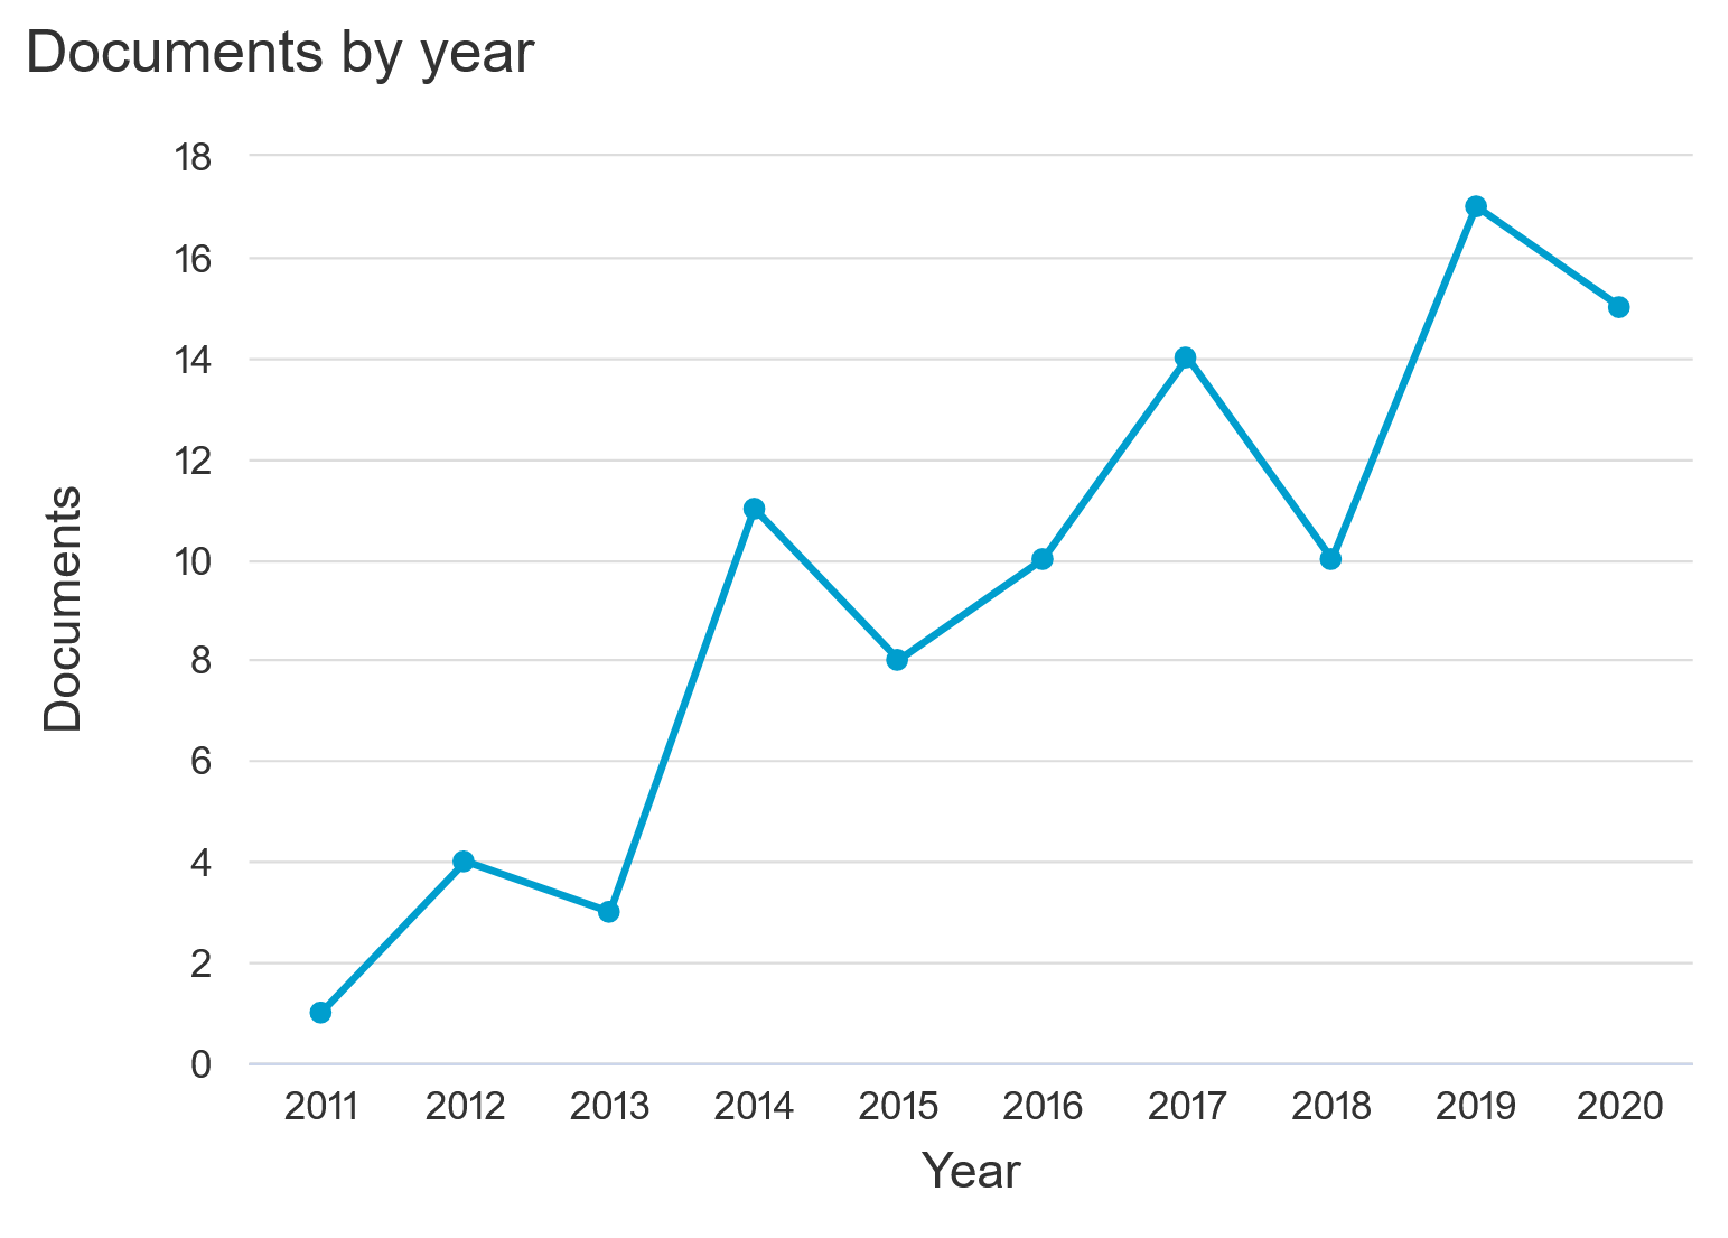
\includegraphics[width=\textwidth]{figures/chap-2/crisis-informatic-hist.pdf}
    \caption{Timelime of the volume of contributions per years for the crisis informatic domain. The year 2021 is excluded because the year is not complete at the time of writing.}
    \label{literature:crisis-informatic-hist}
\end{figure}

The network provided by VOSviewer (Figure~\ref{literature:crisis-informatic-overlay}) do not reveal any significant cluster of keywords, which is not surprising considering the youth of the domain.
However, the timeline of publication (represented by the color variation) provides interesting insight on the direction of the domain.
Years around 2016 were mostly focused on data analyses of the different datasets available.
Then, the following years saw the development of more and more automation.
Artificial intelligence, machine learning and natural language processing appeared in that chronological order, coinciding with the progress made in these areas.
More recently, deep learning models to process text and/or images are appearing, as well as new opportunities created by the internet of things and the development of the concept of smart cities.
It is also very interesting to observe that social sciences and computers sciences are completely blended altogether.

\begin{landscape}
    \begin{figure}[htb]
        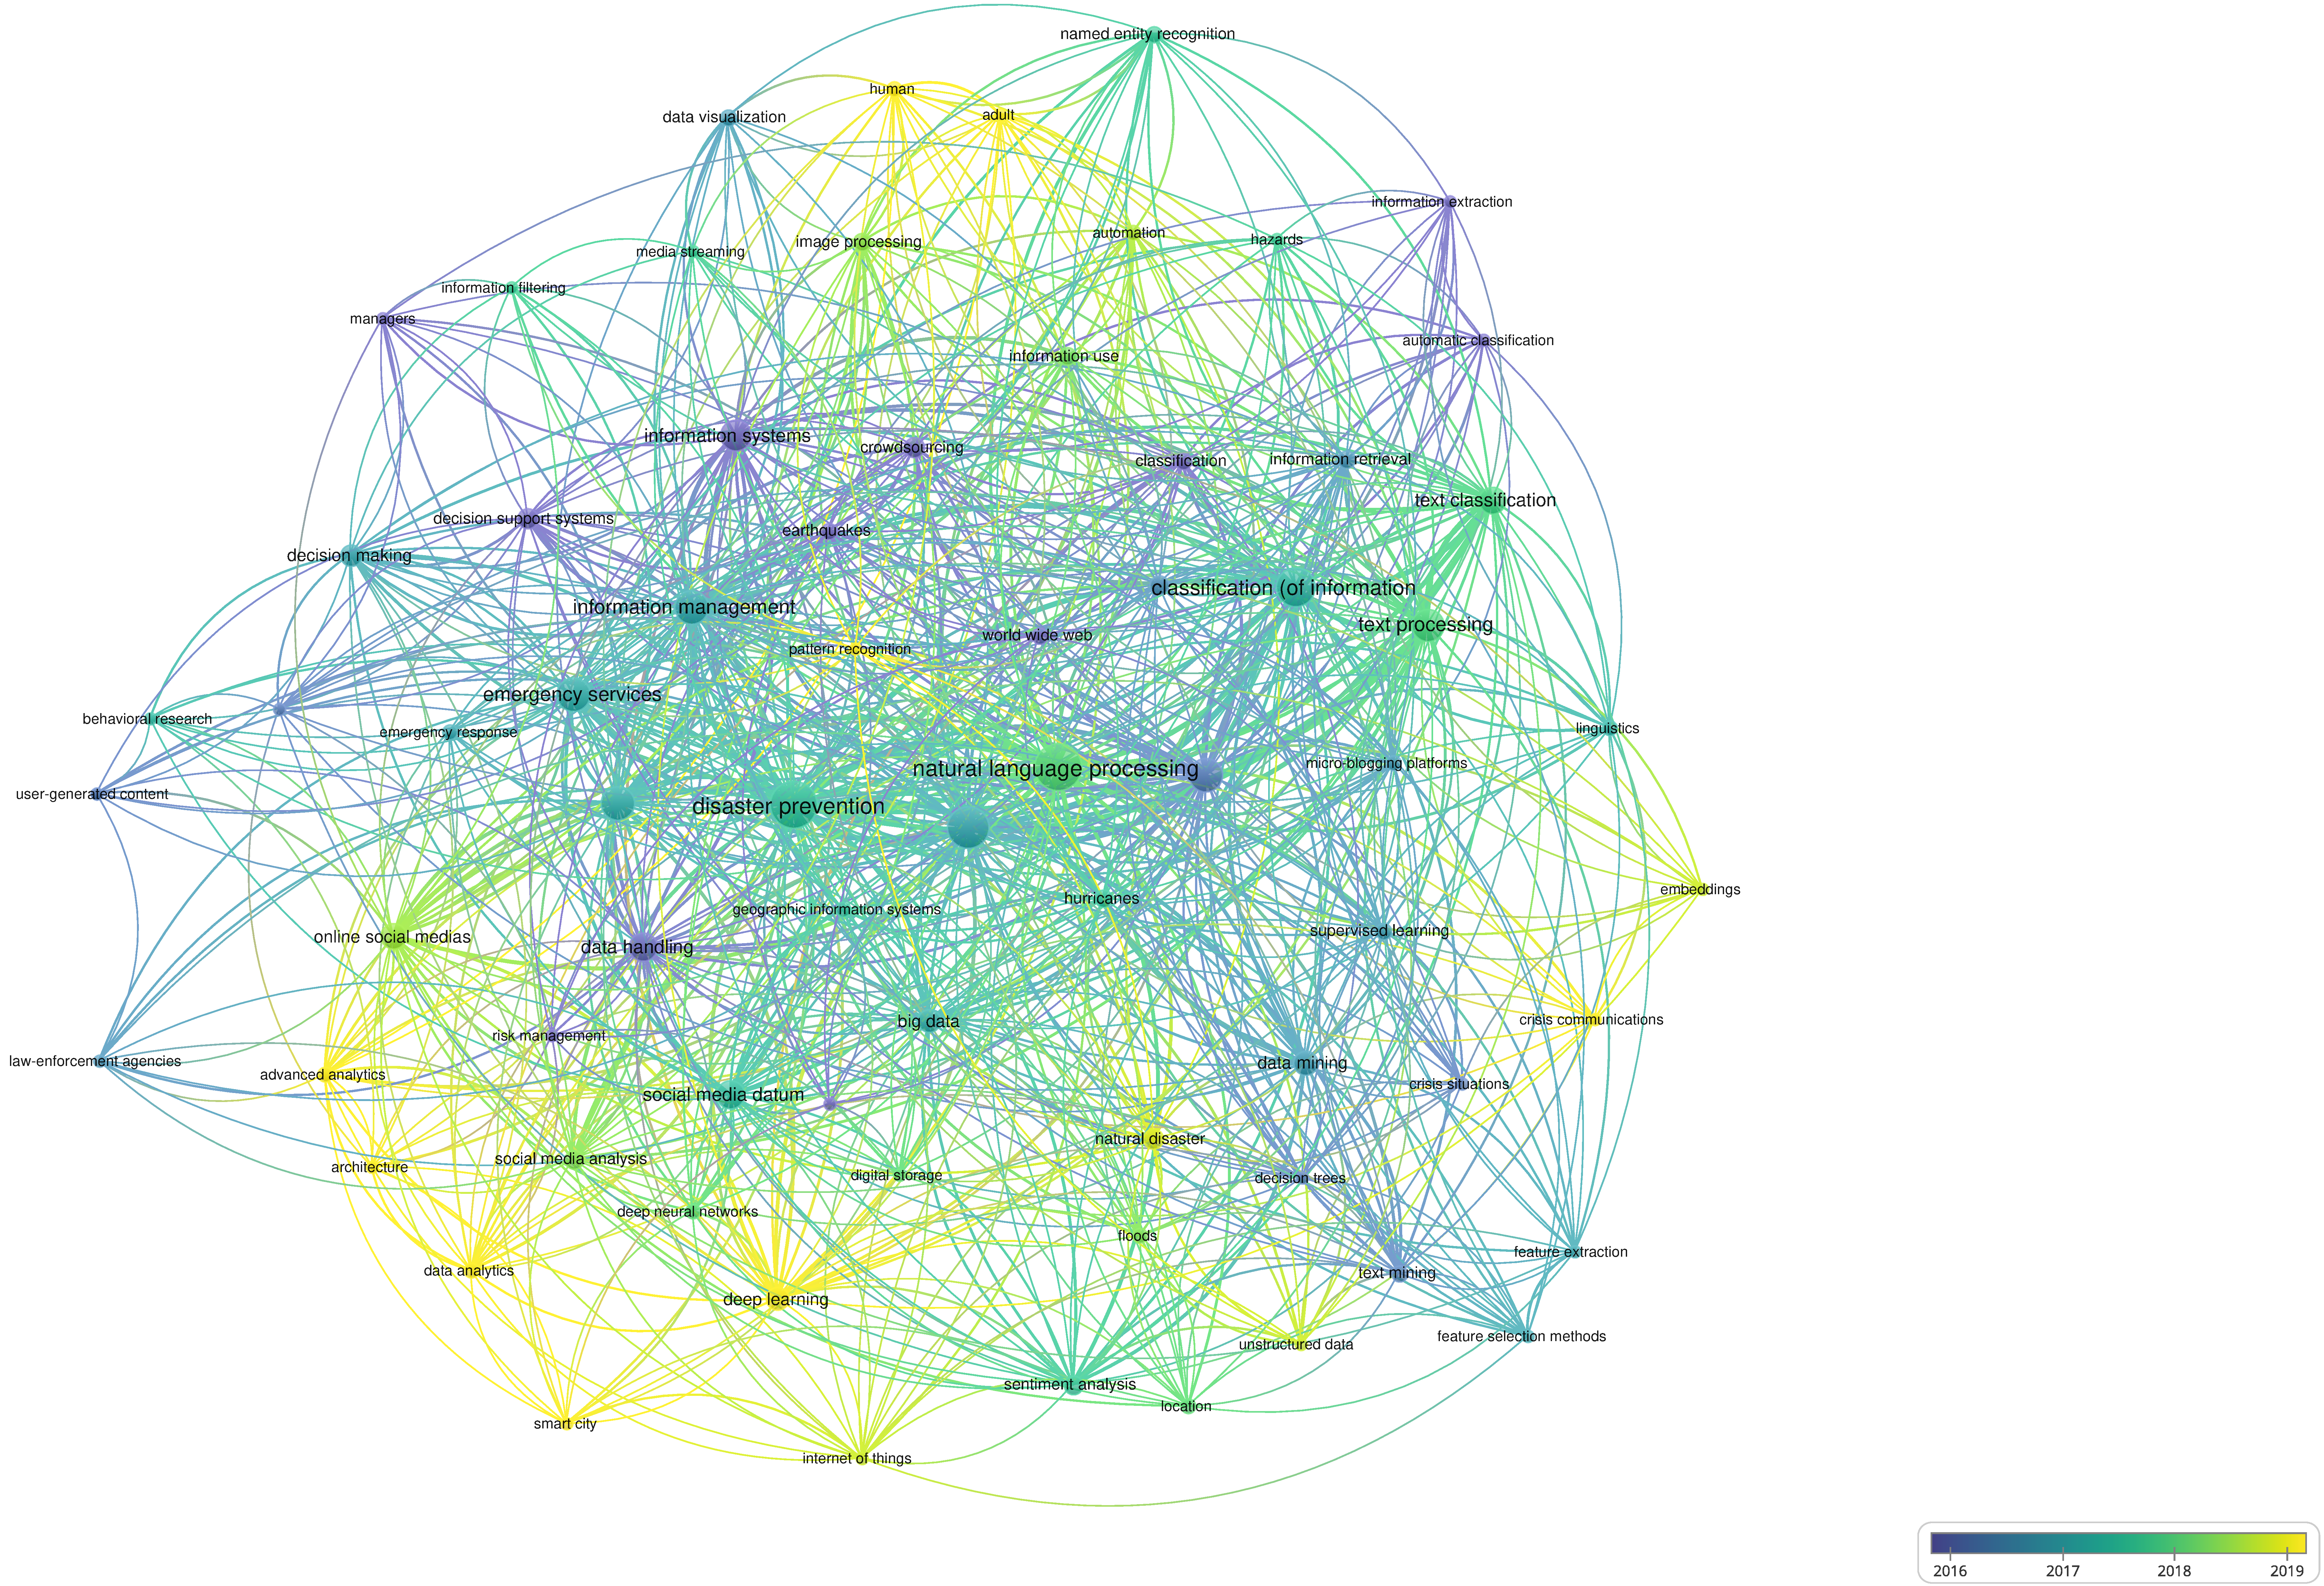
\includegraphics[width=\paperwidth,height=\paperheight,keepaspectratio]{figures/chap-2/crisis-informatic-overlay.pdf}
        \caption{Distribution of keywords with more than 3 occurrences among the articles from the query on crisis informatics. }
        \label{literature:crisis-informatic-overlay}
    \end{figure}
\end{landscape}

The bar diagram (Figure~\ref{literature:crisis-informatic-bar}) provides a better representation of the distribution of the occurrences of the different keywords.
From the most common ones, two areas of interest seem to emerge.
The automatic processing of the data, mostly textual according to the use of \emph{natural language processing} and \emph{text processing} is no more important than the use of this automation.
\emph{Disaster prevention}, \emph{situation awareness}, \emph{information management} and \emph{emergency services} highlight the importance of the applications of the results.

\begin{figure}[htb]
    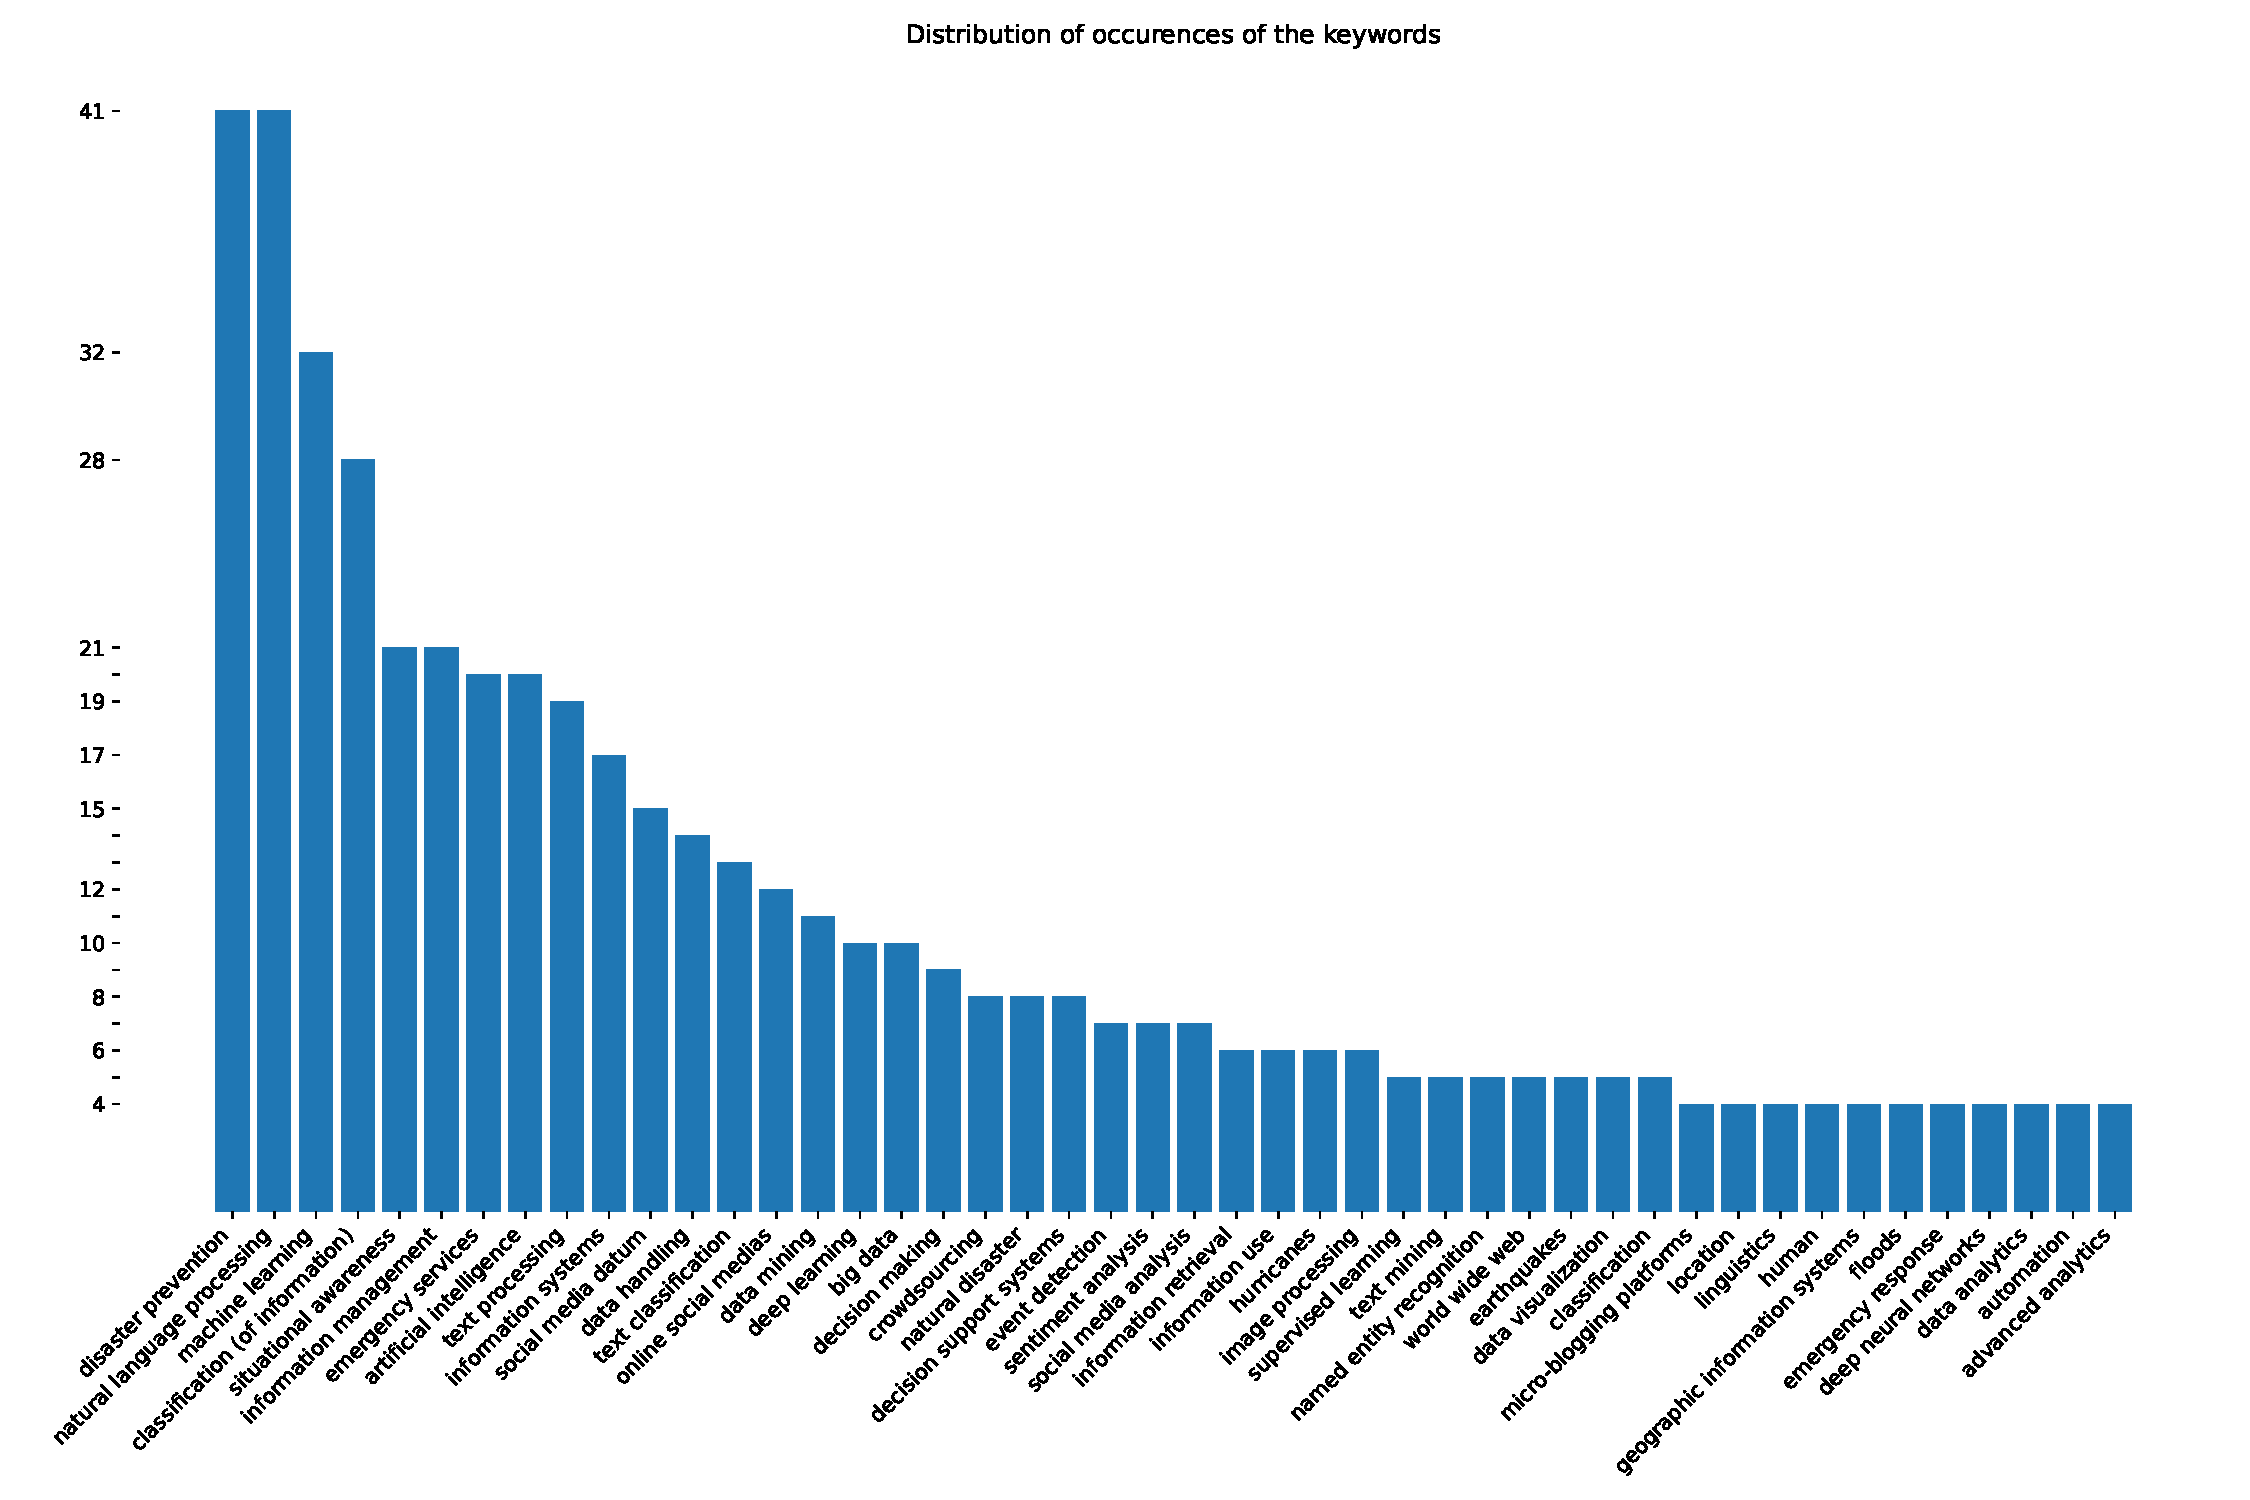
\includegraphics[width=\textwidth]{figures/chap-2/crisis-informatic-bar.pdf}
    \caption{Distribution of keywords with more than 3 occurrences among the articles from the query on crisis informatics. }
    \label{literature:crisis-informatic-bar}
\end{figure}

As mentioned in the first chapter, automatically processing the content of social media to extract information is a new and promising scientific venue.
Thus, many attempted to create systems to achieve this goal, proposing features to improve systems' usability.
Overview of the different attempts and their feature, to identify what have been done in this area.
Table~\ref{table:crisis-informatic-main-articles} presents the results of the previous query that mention a processing system that uses social media as a data source and that have been cited at least ten times are shown.
From these main systems, were extracted the main features presented by their authors.

Among the features identified, the trend towards automation observed earlier is still clear.
The first works present systems that use crowdsourcing to identify relevant information from messages posted on social media
(\cite{schulzCrisisInformationManagement2012, backfriedOpenSourceIntelligence2012,imranAIDRArtificialIntelligence2014}).
The following works were interested in automating the previous tasks, presumably to reduce the dependence on human actors and to improve the processing of the important amount of data.
Problems related to the detection of occurence of events and their related information on social media, have been explored using different approaches (\cite{imranAIDRArtificialIntelligence2014,middletonRealtimeCrisisMapping2014,avvenutiEARSEarthquakeAlert2014, gibsonCombiningBigSocial2014}).
In parallel, experiments were conducted to identify the best ways to organize and disseminate the information obtained (\cite{middletonRealtimeCrisisMapping2014,huangDisasterMapperCyberGISFramework2015,avvenutiPullingInformationSocial2016,grunder-fahrerTopicsTopicalPhases2018}).
Building on its successes, the field has continued to develop by relying on other available data formats and in particular images (\cite{alamImage4ActOnlineSocial2017,nguyenAutomaticImageFiltering2017,agarwalCrisisDIASMultimodalDamage2020}).
Beyond the data, new questions have emerged, following feedback from the emergency departments involved in the experiments.
The detection of sub-events and of the different concerns of the impacted population are added to the results of previous works (\cite{wuStreamExplorerMultiStageSystem2018,raginiBigDataAnalytics2018,grunder-fahrerTopicsTopicalPhases2018}).
More recently, teams with a broader vision are interested in the integration of such systems within the connected city (\cite{shahDisasterResilientSmart2019}).
The multiplication of sources and formats naturally leads to the need for unified processing methods for data and fusion of information obtained by the different channels (\cite{alamDescriptiveVisualSummaries2020}).

\begin{table}[bp]
    \centering
    \renewcommand{\arraystretch}{1.5}
    \caption{Articles retrieved from the previous request which propose social media processing systems or methods with at least 10 citations.}
    \begin{tabular}{m{0.3\textwidth} m{0.2\textwidth} m{0.5\textwidth}}
        Reference                                       & Type of event studied & Features                                                 \\ [0.5ex]
        \toprule
        \cite{schulzCrisisInformationManagement2012}    & None                  & Crowdsourcing                                            \\
        \cite{backfriedOpenSourceIntelligence2012}      & None                  & Crowdsourcing, Automatic processing                      \\
        \cite{imranAIDRArtificialIntelligence2014}      & None                  & Crowdsourcing, Information categories, Message filtering \\
        \cite{middletonRealtimeCrisisMapping2014}       & None                  & Common Operational Picture, Location inference           \\
        \cite{avvenutiEARSEarthquakeAlert2014}          & Earthquake            & Event detection                                          \\
        \cite{gibsonCombiningBigSocial2014}             & None                  & Formal concept analysis, Rule-based method               \\
        \cite{glasgowOurGriefUnspeakable2014}           & None                  & Death-related content detection                          \\
        \cite{huangDisasterMapperCyberGISFramework2015} & None                  & Big Data, Common Operational Picture                     \\
        \cite{avvenutiPullingInformationSocial2016}     & Earthquake, Flooding  & Event detection, Message filtering, Disaster management  \\
        \cite{alamImage4ActOnlineSocial2017}            & None                  & Image processing, Infrastructure damage                  \\
        \cite{fersiniEarthquakeManagementDecision2017}  & Earthquake            & Message filtering, Information management                \\
        \cite{nguyenAutomaticImageFiltering2017}        & None                  & Image processing, De-duplication, Image filtering        \\
        \cite{raginiBigDataAnalytics2018}               & Flooding              & Sentiment analysis                                       \\
        \cite{shahDisasterResilientSmart2019}           & Earthquake, Tsunami   & Smart Cities, IoT integration                            \\
        \cite{grunder-fahrerTopicsTopicalPhases2018}    & None                  & Topic modeling, Disaster management                      \\
        \cite{wuStreamExplorerMultiStageSystem2018}     & None                  & Subevent detection, Clustering                           \\
        \cite{agarwalCrisisDIASMultimodalDamage2020}    & None                  & Damage identification, Severity detection                \\
        \cite{alamDescriptiveVisualSummaries2020}       & Hurricane             & Information fusion                                       \\
        \bottomrule
    \end{tabular}
    \label{table:crisis-informatic-main-articles}
\end{table}

This introductory section presented previous works around crisis informatics.
More particularly, it highlighted the development of the field over time.
This is directly reflected in the different systems developed and their features.
An interesting trend to note is the move towards more and more automation in systems.
First using crowdsourcing for initial data labeling, the following systems used machine learning to classify the data into different categories.
Later, automation was further extended to other valuable data types and ways to merge the information acquired.

\section{Decision making in crisis situation}
This part of the literature review explores the bibliographic context aroung the first sub problematic: What information that can be obtained from social media is relevant to the decisiom makers in crisis response?
Specifically, its looks at answers at the question: \emph{what is the decision-making context in emergency situations?}

Decision making is at the heart of the response during a disaster.
Ideally, the right decisions need to be made at the right time.
In order to get as close as possible of that unrealistic expectation, it is best to first
understand: (i) the previous attempts to understand the word of decisions makers and
(ii) what hinders them in the performance of their tasks and their main pains?

\subsection{Organization of information during crises: crisis situation models}
Crisis management is as ancient as crises themselves.
Thus, many tackled the problems in this area.
With the advent of computers as a way to delegate tasks, many have thought of delegating some of the crisis management to machines.
However, managing this information require at first to build representations (or abstractions) of crises for computers.
Consequently, ontologies and information models emerged to represent the informational concepts manipulated during an emergency situation.
This sub-section aims at retrieving from the literature the different key informational concepts, useful for decision makers during crisis response.

The request run on Scopus is as follow:
\begin{itemize}
    \item SUBJAREA(comp)
    \item AND (TITLE-ABS-KEY ({crisis management} or {crisis response} or {disaster management} or contingency or {disaster response}))
    \item AND (TITLE-ABS-KEY (ontology or metamodel))
    \item AND (EXCLUDE (DOCTYPE,"re") OR EXCLUDE (DOCTYPE,"cr"))
\end{itemize}

The request returns papers that:
\begin{itemize}
    \item Are in the computer science domain, as this domain contains both the AI and Information Systems domains.
    \item Are centered around crises|disasters management|response or contingency plans.
    \item That present systems that process data
    \item Papers that present conference tracks and reviews are excluded.
\end{itemize}

The request returns 205 documents, published between 1998 and 2021.
Figure~\ref{literature:situation-models-hist} shows the evolution of the volume of publication between 1998 and 2020.
The field has emerged around 2000 and built momentum during ten years to reach a plateau of fifteen articles on average per years.
The domain developped in order to organize the data, information and knowledge present during crisis events.
To achieve this goal, representions of the different concepts involved during such events were needed.
Two paths to represent these concepts have been taken: ontologies and metamodels.
Ontologies and metamodels are very close concepts.
Both methods aim at creating a controlled vocabulary to define the entities and their relations in a given domain.
The difference between the two methos happens at the grammar used for the vocabulary.
Metamodels usually use a formal and common grammar (a modelisation language such as UML) to ease the distribution and development of these representation.
Metamodels, as the backbone of model driven engineering, tend to be developped with interoperability between different systems in mind.
Thus the use of common tools to represent concepts between the engineers.
Ontologies, on the other hand, use their own grammar for the entities that its define.
As mentioned in the first chapter, crises are a were wide concept and the creation of ontologies or metamodels of crisis situations is a very challenging task.
Thus, many ontologies and metamodels have been created to represent different aspects of crisis management.

\begin{figure}[htb]
    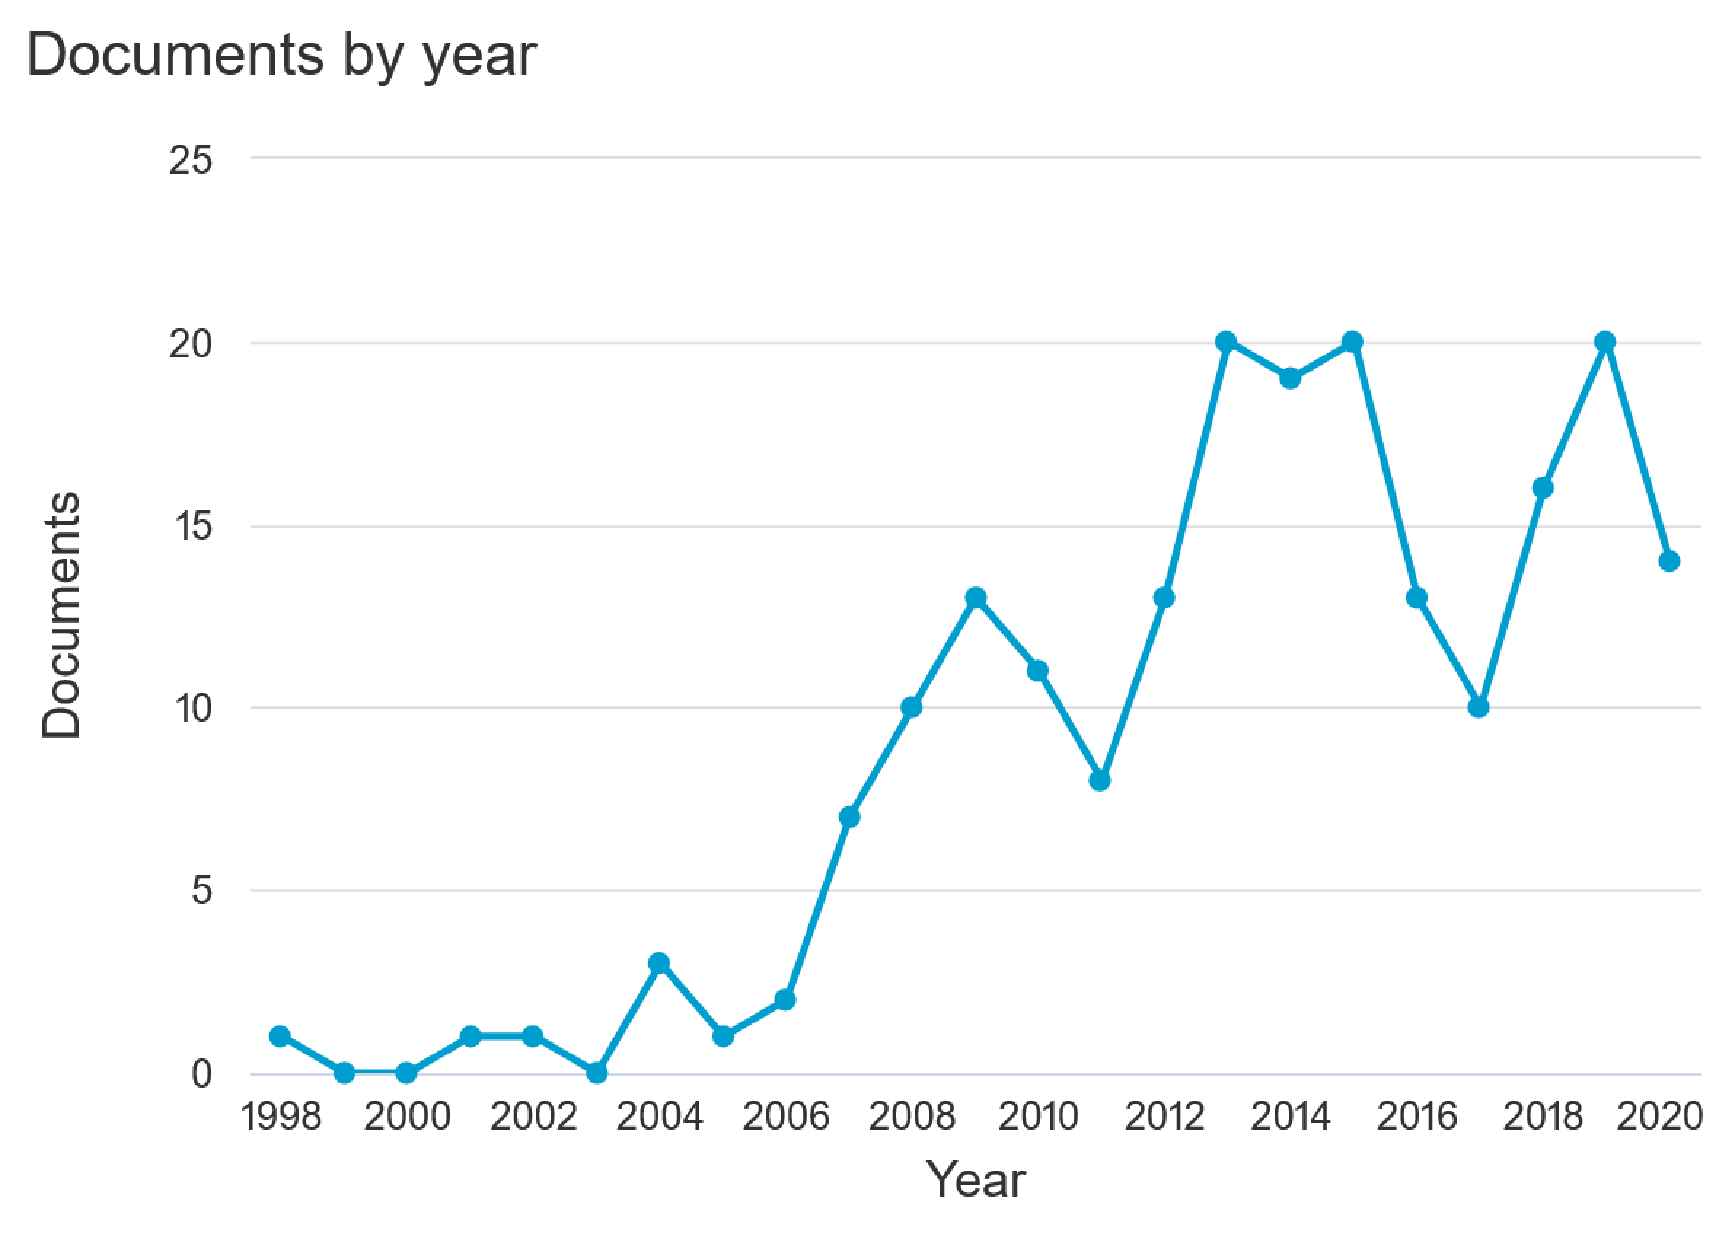
\includegraphics[width=\textwidth]{figures/chap-2/situation-models-hist.pdf}
    \caption{Timelime of the volume of contributions per years for the crisis-situation models domain. The year 2021 is excluded because the year is not complete at the time of writing.}
    \label{literature:situation-models-hist}
\end{figure}

Following the same methodology as in the previous section, Figure~\ref{literature:situation-models-overlay} provides a visual of the evolution over time of the different keywords used in the fetched articles.
The overlay indicates three clusters: a major one and two smaller ones.
One is related to genes and the other one is related to supply chains and infrastructures.
The one related to genes is a cluster of outliers, composed of 7 articles from the medical field.
The second cluster is also composed of few articles centered around ontologies for the petroleum sector.
The main cluster however, is more centered on the topic of this literature review.
As in the previous section, the evolution (represented by the color variation) of the keywords hint at the direction of the domain over time.

\begin{landscape}
    \begin{figure}[htb]
        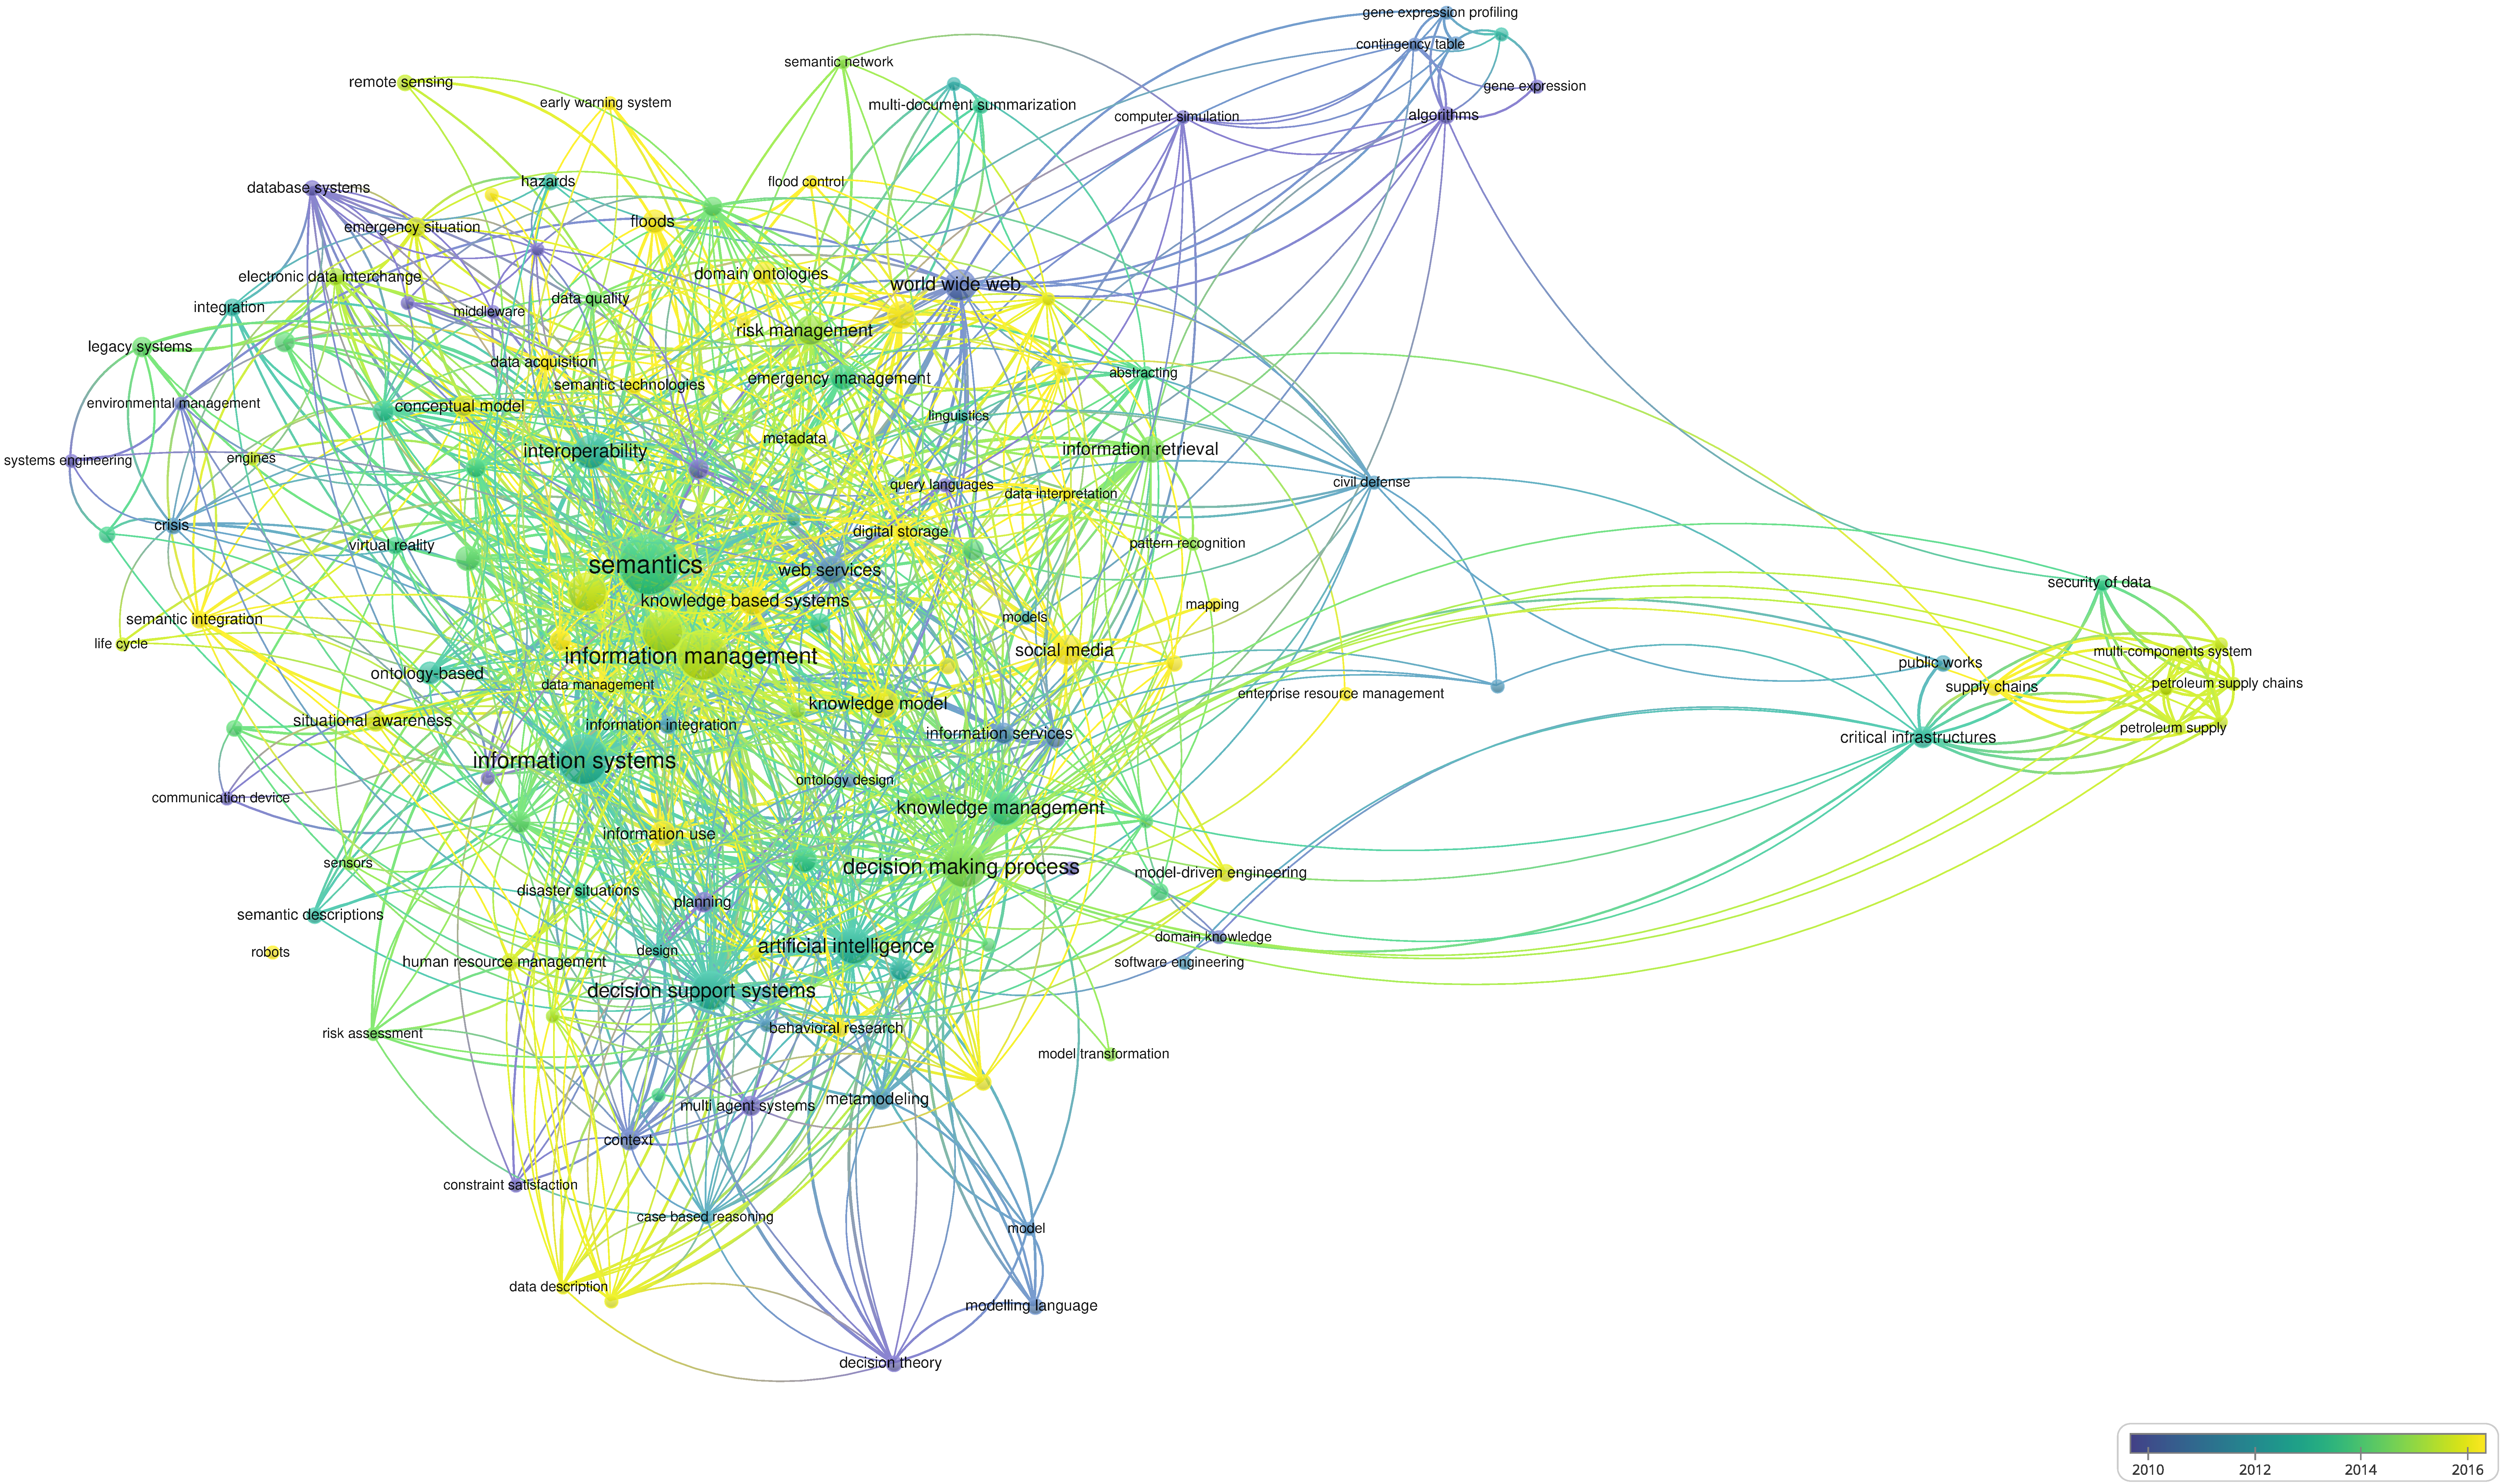
\includegraphics[width=\paperwidth,height=\paperheight,keepaspectratio]{figures/chap-2/situation-models-overlay.pdf}
        \caption{Distribution of keywords with more than 3 occurrences among the articles from the query on crisis-situation models.}
        \label{literature:situation-models-overlay}
    \end{figure}
\end{landscape}

Unlike the query, the overlay spans from 2010 to 2016. This is because the overlay does not include all keywords, but only those that appear in at least 3 different articles.
By cross-checking this information with the previous histogram, one understands the reason for this short period.
For many years the number of publications was relatively low, and apparently without any real consensus among the keywords.
If this is understandable at the beginning of a field, this explanation does not explain the stop of the overlay from 2016.
However, using again the histogram, one notices that the domain loses popularity from 2015 onwards to return to its previous level around 2018.
It is possible to hypothesize that it is this loss of interest that has led to the result observed on the overlay.

Despite this short span covered, it is possible to identify trends in keywords use somehow similar to the ones in crisis informatic.
The older keywords used, such as "SOA", "simulation", "multi agent systems" and "systems engineering" show an interest centered around the core of what were used ontologies and metamodels for: model driven engineering and information management.
Then, the field knew a pic of interest, as the previous histogram show.
This period reflects on Figure~\ref{literature:situation-models-bar}, where one can observe that most of the most importants keywords are located between 2012 and 2014.
As explained previously, the years between 2021 and 2014 were indeed the most prolific.
These years were mostly focused on the idea of crisis management systems, powered by artifical intelligence for decision support.
Artificial intelligence would automatically create the information representations needed by systems.
As these representations would have been written in a common fashion, these systems would have been able to quickly adapt to new representations, providing greater interoperability.
After this period, the interest in the field decrease a few, before coming back with new approaches.
Knowledge based systems and knowledge management started to appear, as well as a reborn of metamodel and ontologies creation, powered by improvements in machine learning.

\begin{figure}[htb]
    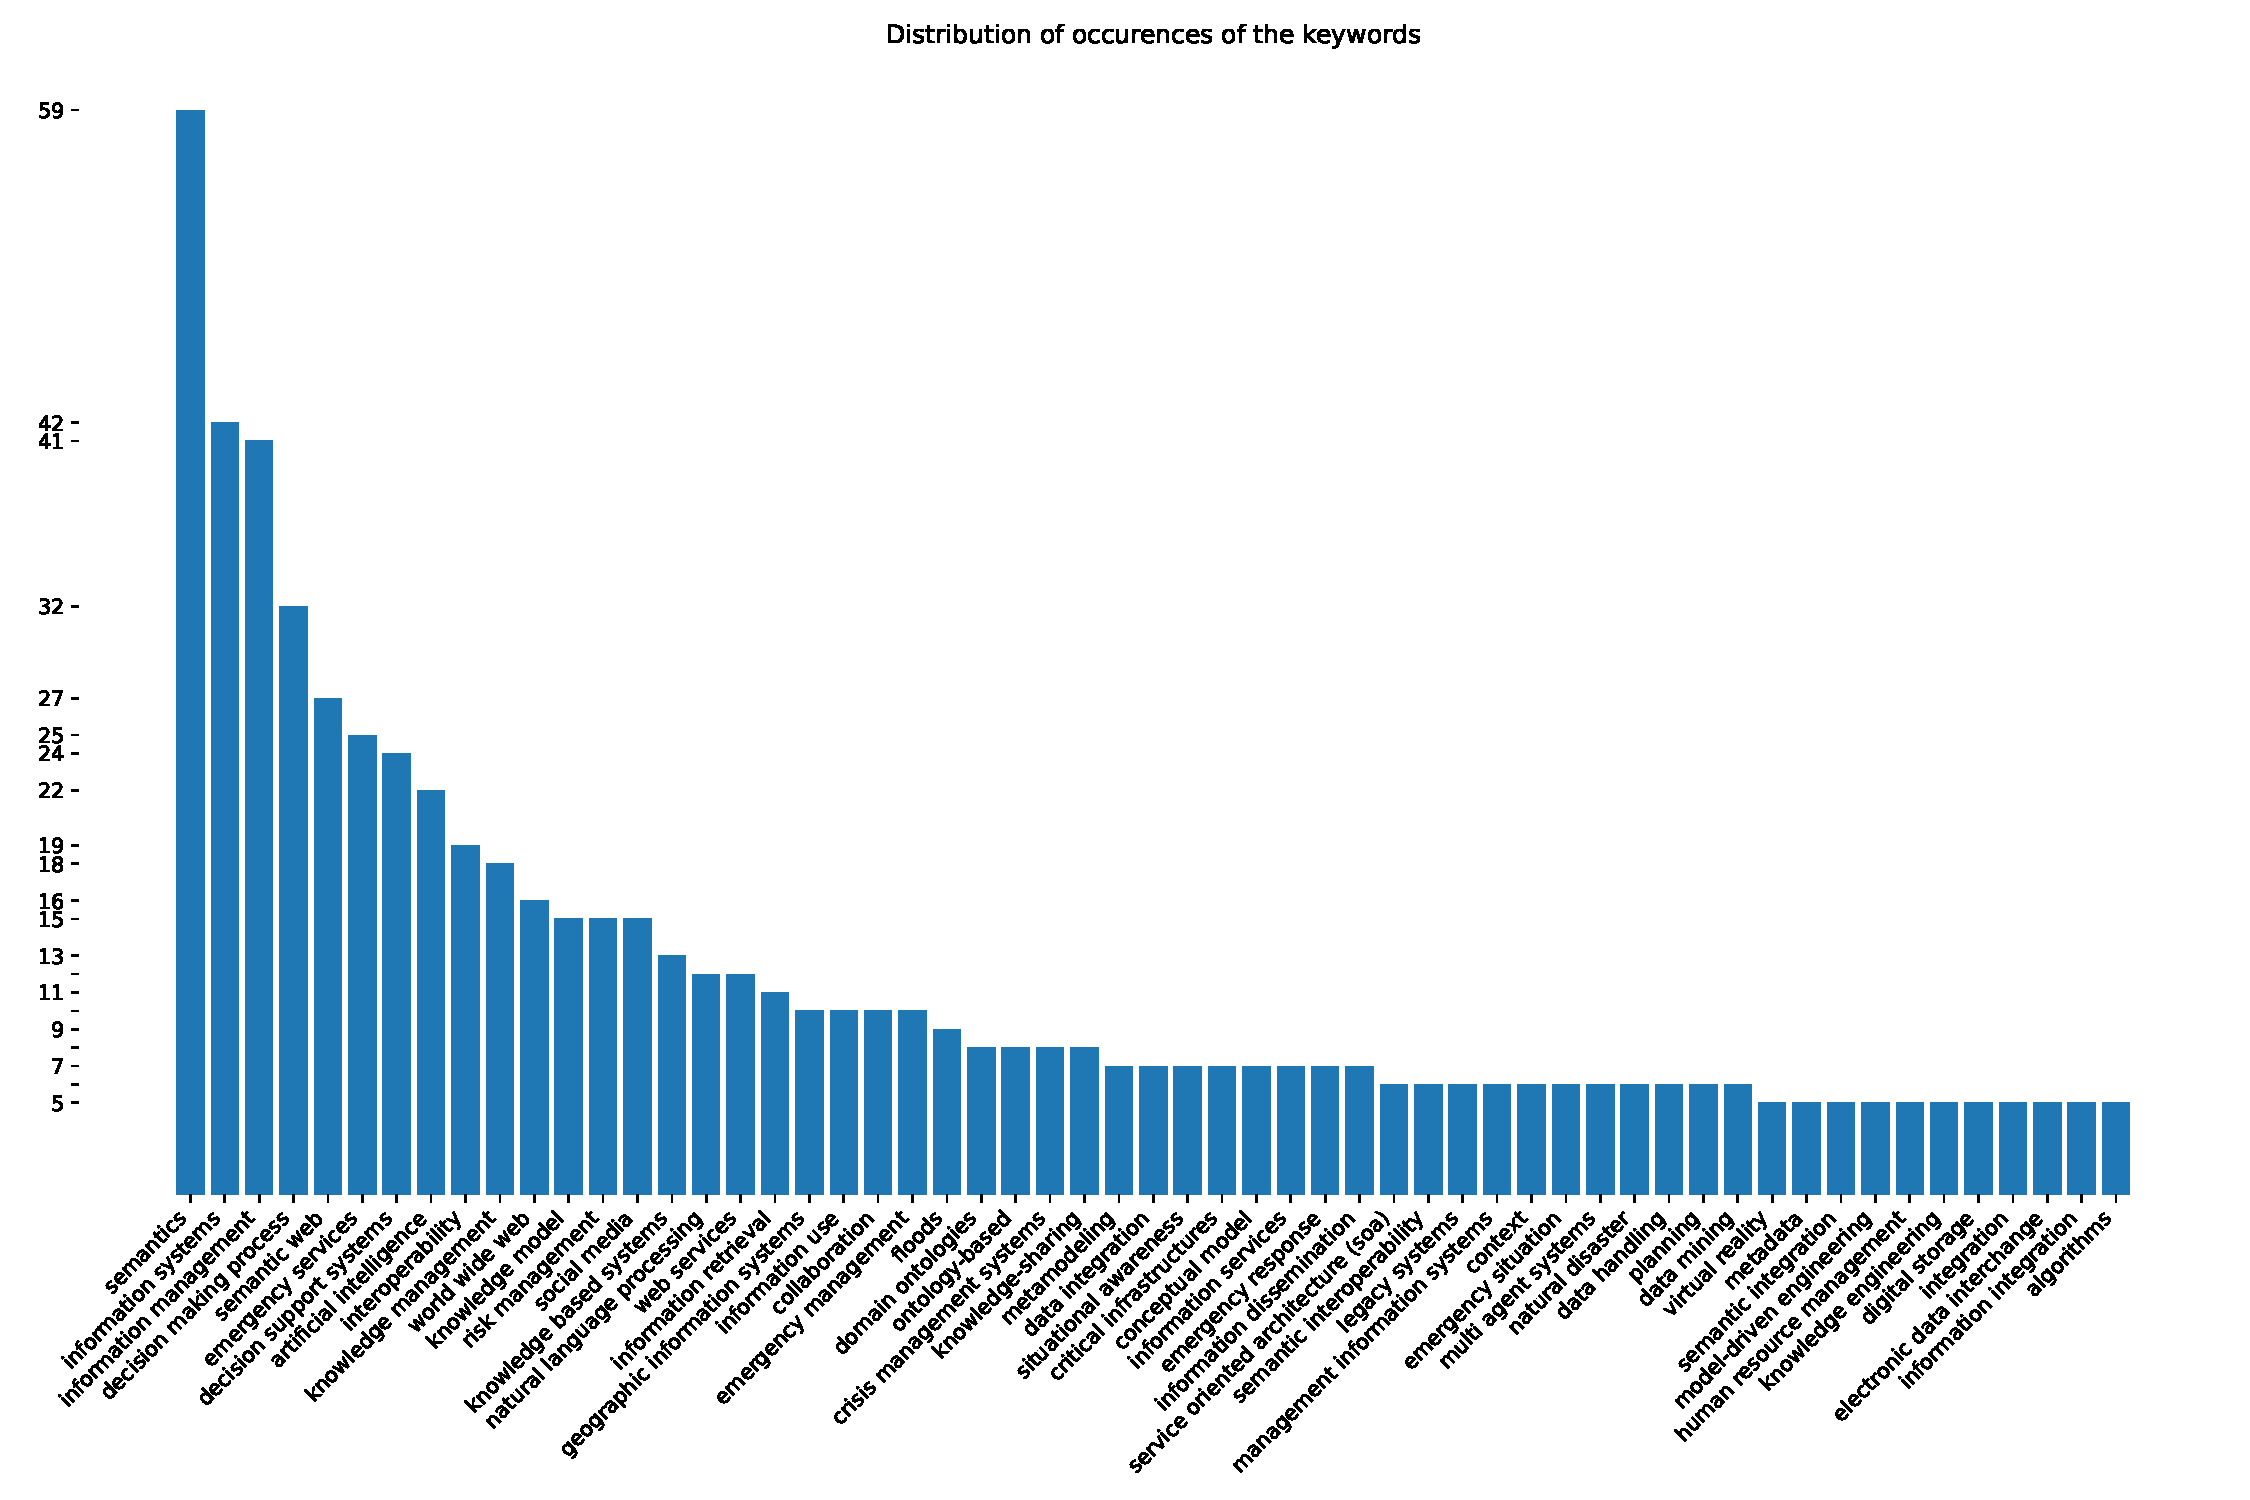
\includegraphics[width=\textwidth]{figures/chap-2/situation-models-bar.pdf}
    \caption{Distribution of keywords with more than 4 occurrences among the articles from the query on crisis-situation models.}
    \label{literature:situation-models-bar}
\end{figure}

In association with the previous qualitative review of the field, Table~\ref{table:situation-models-main-articles} presents the decision makers needs identified in the articles from the previous request with at least 25 citations.
Duplicates and unrelated articles (e.g. gene ontologies) are also excluded.
This review of the main articles highlight the diversity of approaches covered by ontologies and metamodels.
Some of these ontologies are event specific (\cite{xuModelingRepresentationEarthquake2014,qiuIntegratedFloodManagement2017,jungOntologydrivenSlopeModeling2015}).
While these models are effective at dealing with the event they are designed for, most of their concept representations do not fit with other kind of events.

Collaboration between the actors is, as presented in the introductory chapter, a matter of interest for crisis management organizations.
Thus (\cite{benabenMetamodelItsOntology2008b}) and (\cite{othmanDevelopmentValidationDisaster2014b}) propose metamodels to represent the collaboration between several actors, independantly of the type of crisis.

Others have also focused on emergency organization and proposed ways to improve their functioning.
\cite{chouOntologyDevelopingWeb2011} proposed a way to automatically create websites to dissemination information related to an ongoing event.
As reports are an important concerns and participate to information overload, \cite{liOntologyenrichedMultiDocumentSummarization2010} created an ontology to assist in report summarization.
Disaster management software are inherently complex. Thus, \cite{babitskiSoKNOSUsingSemantic2011} proposed an ontology to assist in their development and another to assess their functionalities.
As disaster management systems grow, they become intricated and complex. \cite{madniSystemsIntegrationKey2014} proposed an ontology to facilitate their integration into a functioning system of systems.

All the systems mentioned above require data.
Fortunately, sensors are excellent ways to keep emergency responders informed of certain caracteristics of their environment.
\cite{posladSemanticIoTEarly2015} and \cite{babitskiOntologybasedIntegrationSensor2009} proposed ontologies to better integrate sensors data into crisis cells.
Finally, another type of sensor considered are humans, acting as social sensors whose data can be automatically gathered from social media plateforms.
\cite{purohitIdentifyingSeekersSuppliers2014} proposed an ontology to identify victims requests and volunteers capabilities from tweets.
As being able to geolocate the individual behind a post allows better actionability for emergency services, \cite{ghahremanlouGeotaggingTwitterMessages2014} built an ontology to help solve this issue.

\begin{table}[bp]
    \centering
    \renewcommand{\arraystretch}{1.5}
    \caption{Articles retrieved from the previous request which propose social media processing systems or methods with at least 25 citations.}
    \begin{tabular}{m{0.25\textwidth} m{0.75\textwidth}}
        Reference                                               & Decision makers needs adressed         \\ [0.5ex]
        \toprule
        \cite{benabenMetamodelItsOntology2008b}                 & Collaboration                          \\
        \cite{babitskiOntologybasedIntegrationSensor2009}       & Sensor integration                     \\
        \cite{liOntologyenrichedMultiDocumentSummarization2010} & Reports summarization                  \\
        \cite{babitskiSoKNOSUsingSemantic2011}                  & Disaster management software usability \\
        \cite{chouOntologyDevelopingWeb2011}                    & Automatic web sites creation           \\
        \cite{ghahremanlouGeotaggingTwitterMessages2014}        & Location retrieval                     \\
        \cite{madniSystemsIntegrationKey2014}                   & System integration                     \\
        \cite{othmanDevelopmentValidationDisaster2014b}         & Collaboration                          \\
        \cite{purohitIdentifyingSeekersSuppliers2014}           & Identify victims and volunteers        \\
        \cite{xuModelingRepresentationEarthquake2014}           & Earthquake management                  \\
        \cite{jungOntologydrivenSlopeModeling2015}              & Landslide prevention                   \\
        \cite{posladSemanticIoTEarly2015}                       & Sensor intregration                    \\
        \cite{qiuIntegratedFloodManagement2017}                 & Flood management                       \\
        \bottomrule
    \end{tabular}
    \label{table:situation-models-main-articles}
\end{table}

This part identified the different approaches to model information in crisis response from a decision maker point of view.
Yet, most of these approaches are top-down, and few conducted interviews to directly identify decision makers needs'.
The next section looks at articles in the literature that used a bottom-up approach to identify the aforementioned needs.

\subsection{Business needs of emergency services}
Emergency management teams are tasked with novel and complex decisions.
Information collection is one of the lever that ease decision making and, therefore,
facilitate crisis management.
Knowing what are the different elements that hinders emergency management teams from
achieving their goals and what could ease information gathering is of the utmost importance to improve crisis management.
Researchers in social sciences have been interested in the study of these pain points.
This section aims to highlight the main issues identified in the literature.

The executed request is:

\begin{itemize}
    \item TITLE-ABS-KEY({information gathering} or interview?)
    \item AND TITLE-ABS-KEY({emergency responders} or {Emergency services} or {dispatchers})
    \item AND (LIMIT-TO (SUBJAREA,"SOCI") OR LIMIT-TO (SUBJAREA,"COMP") OR LIMIT-TO (SUBJAREA,"DECI"))
    \item AND (EXCLUDE(DOCTYPE,"re") OR EXCLUDE(DOCTYPE,"cr"))
\end{itemize}

It aims at obtaining articles that:

\begin{itemize}
    \item Mention information gathering or interview in their content and mention emergency responders, dispatchers or emergency services.
    \item Are linked to social sciences, computer sciences or decision sciences.
    \item Papers that present conference tracks and reviews are excluded.
\end{itemize}

The request returns 219 documents, published between 1995 and 2021.
The area follows an increasing trend similar to the other two previous areas.
Interest in the study of emergency services has been growing rapidly since the 2000s.
This interest grew relatively steadily until today, where about 20 articles are published per year on the subject (Figure~\ref{literature:business-needs-hist}).

\begin{figure}[htb]
    \centering
    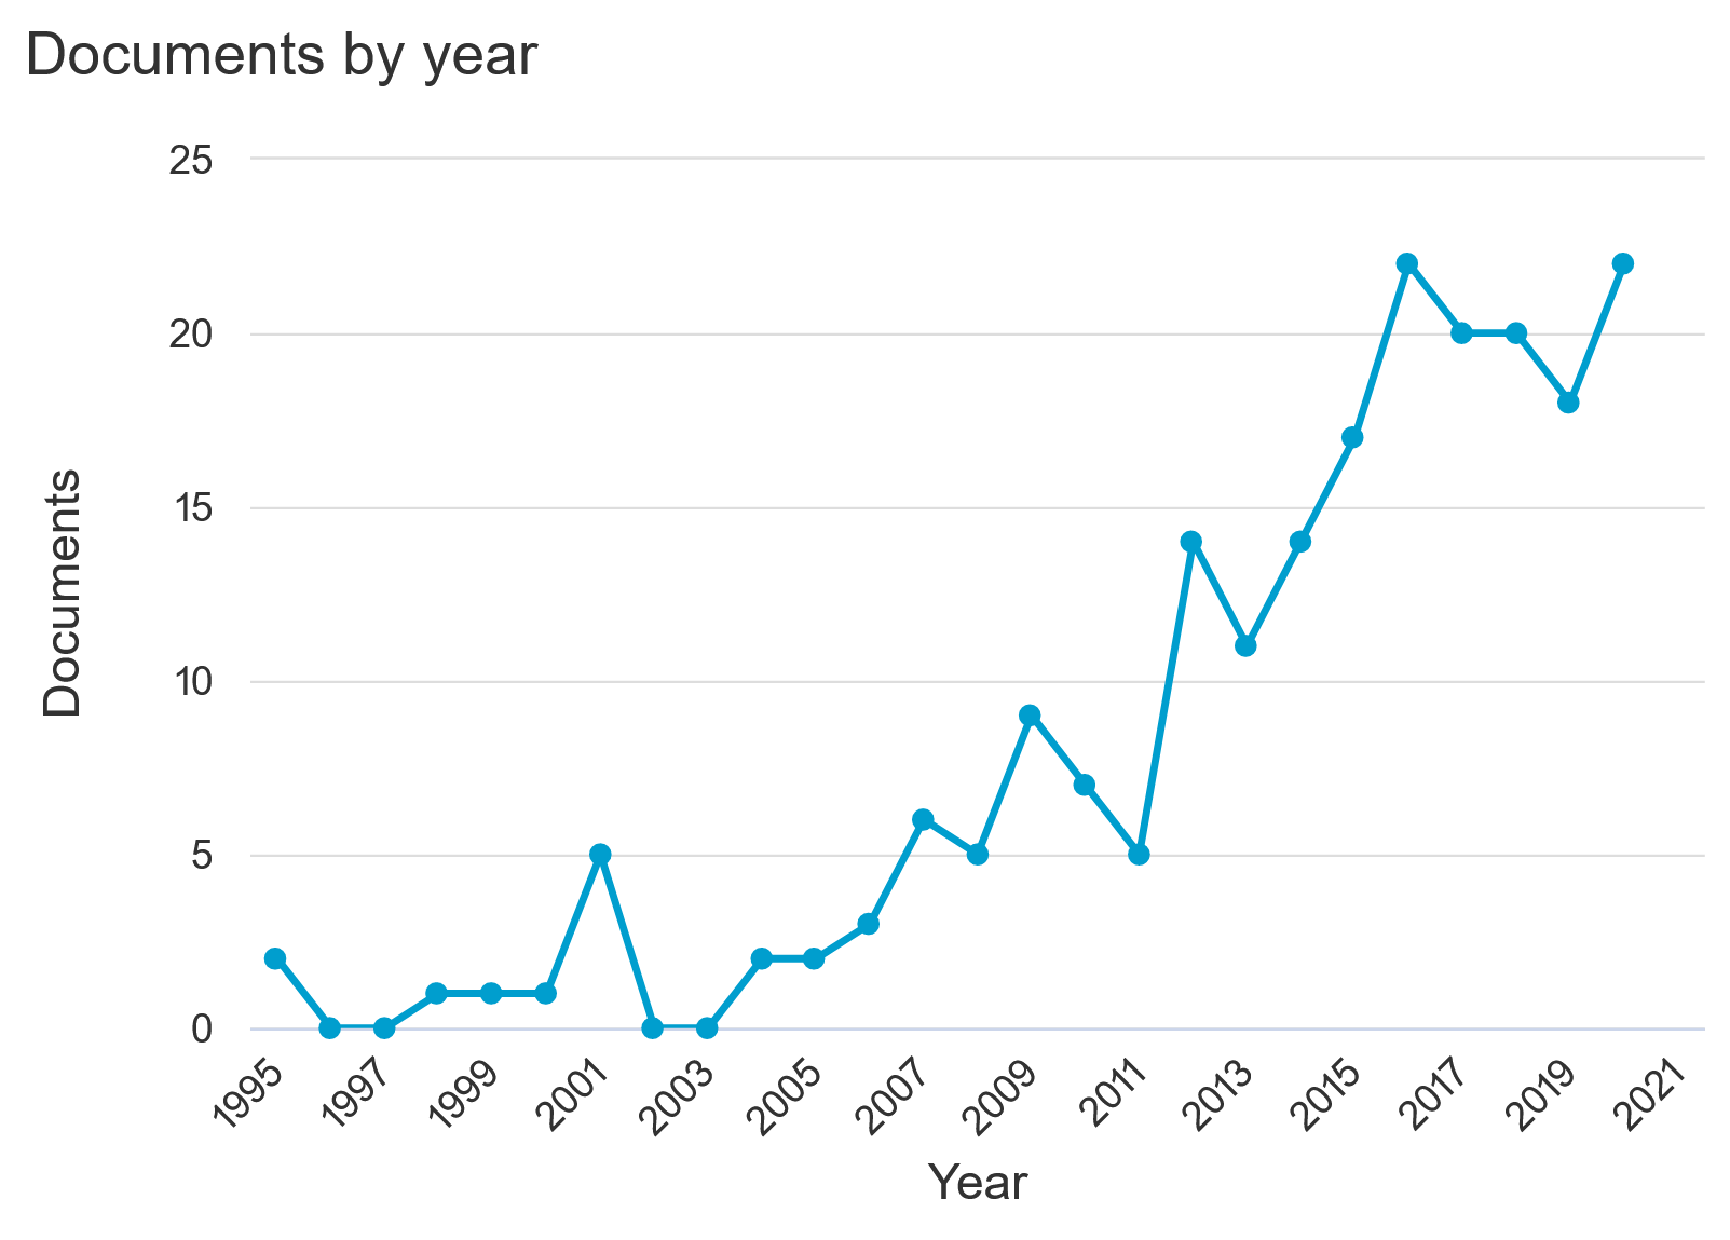
\includegraphics[width=\textwidth]{figures/chap-2/business-needs-hist.pdf}
    \caption{Timelime of the volume of contributions per years for information needs of crisis responders. The year 2021 is excluded because the year is not complete at the time of writing.}
    \label{literature:business-needs-hist}
\end{figure}

The overlay of the keywords generated from the articles retrieved (Figure~\ref{literature:business-needs-overlay}) spans from 2010 to 2018.
It reveals two clusters: one centered on medical issues and another one centered on information systems.
The medical cluster is mainly focused on the well-being of the personnel in charge of the emergency and in particular in their psychological health.
The other cluster is more focused on the information systems of emergency services and in the management of events.
This last one being more in connection with the objective of this manuscript, the next analysis will be focused on it.

\begin{landscape}
    \begin{figure}[htb]
        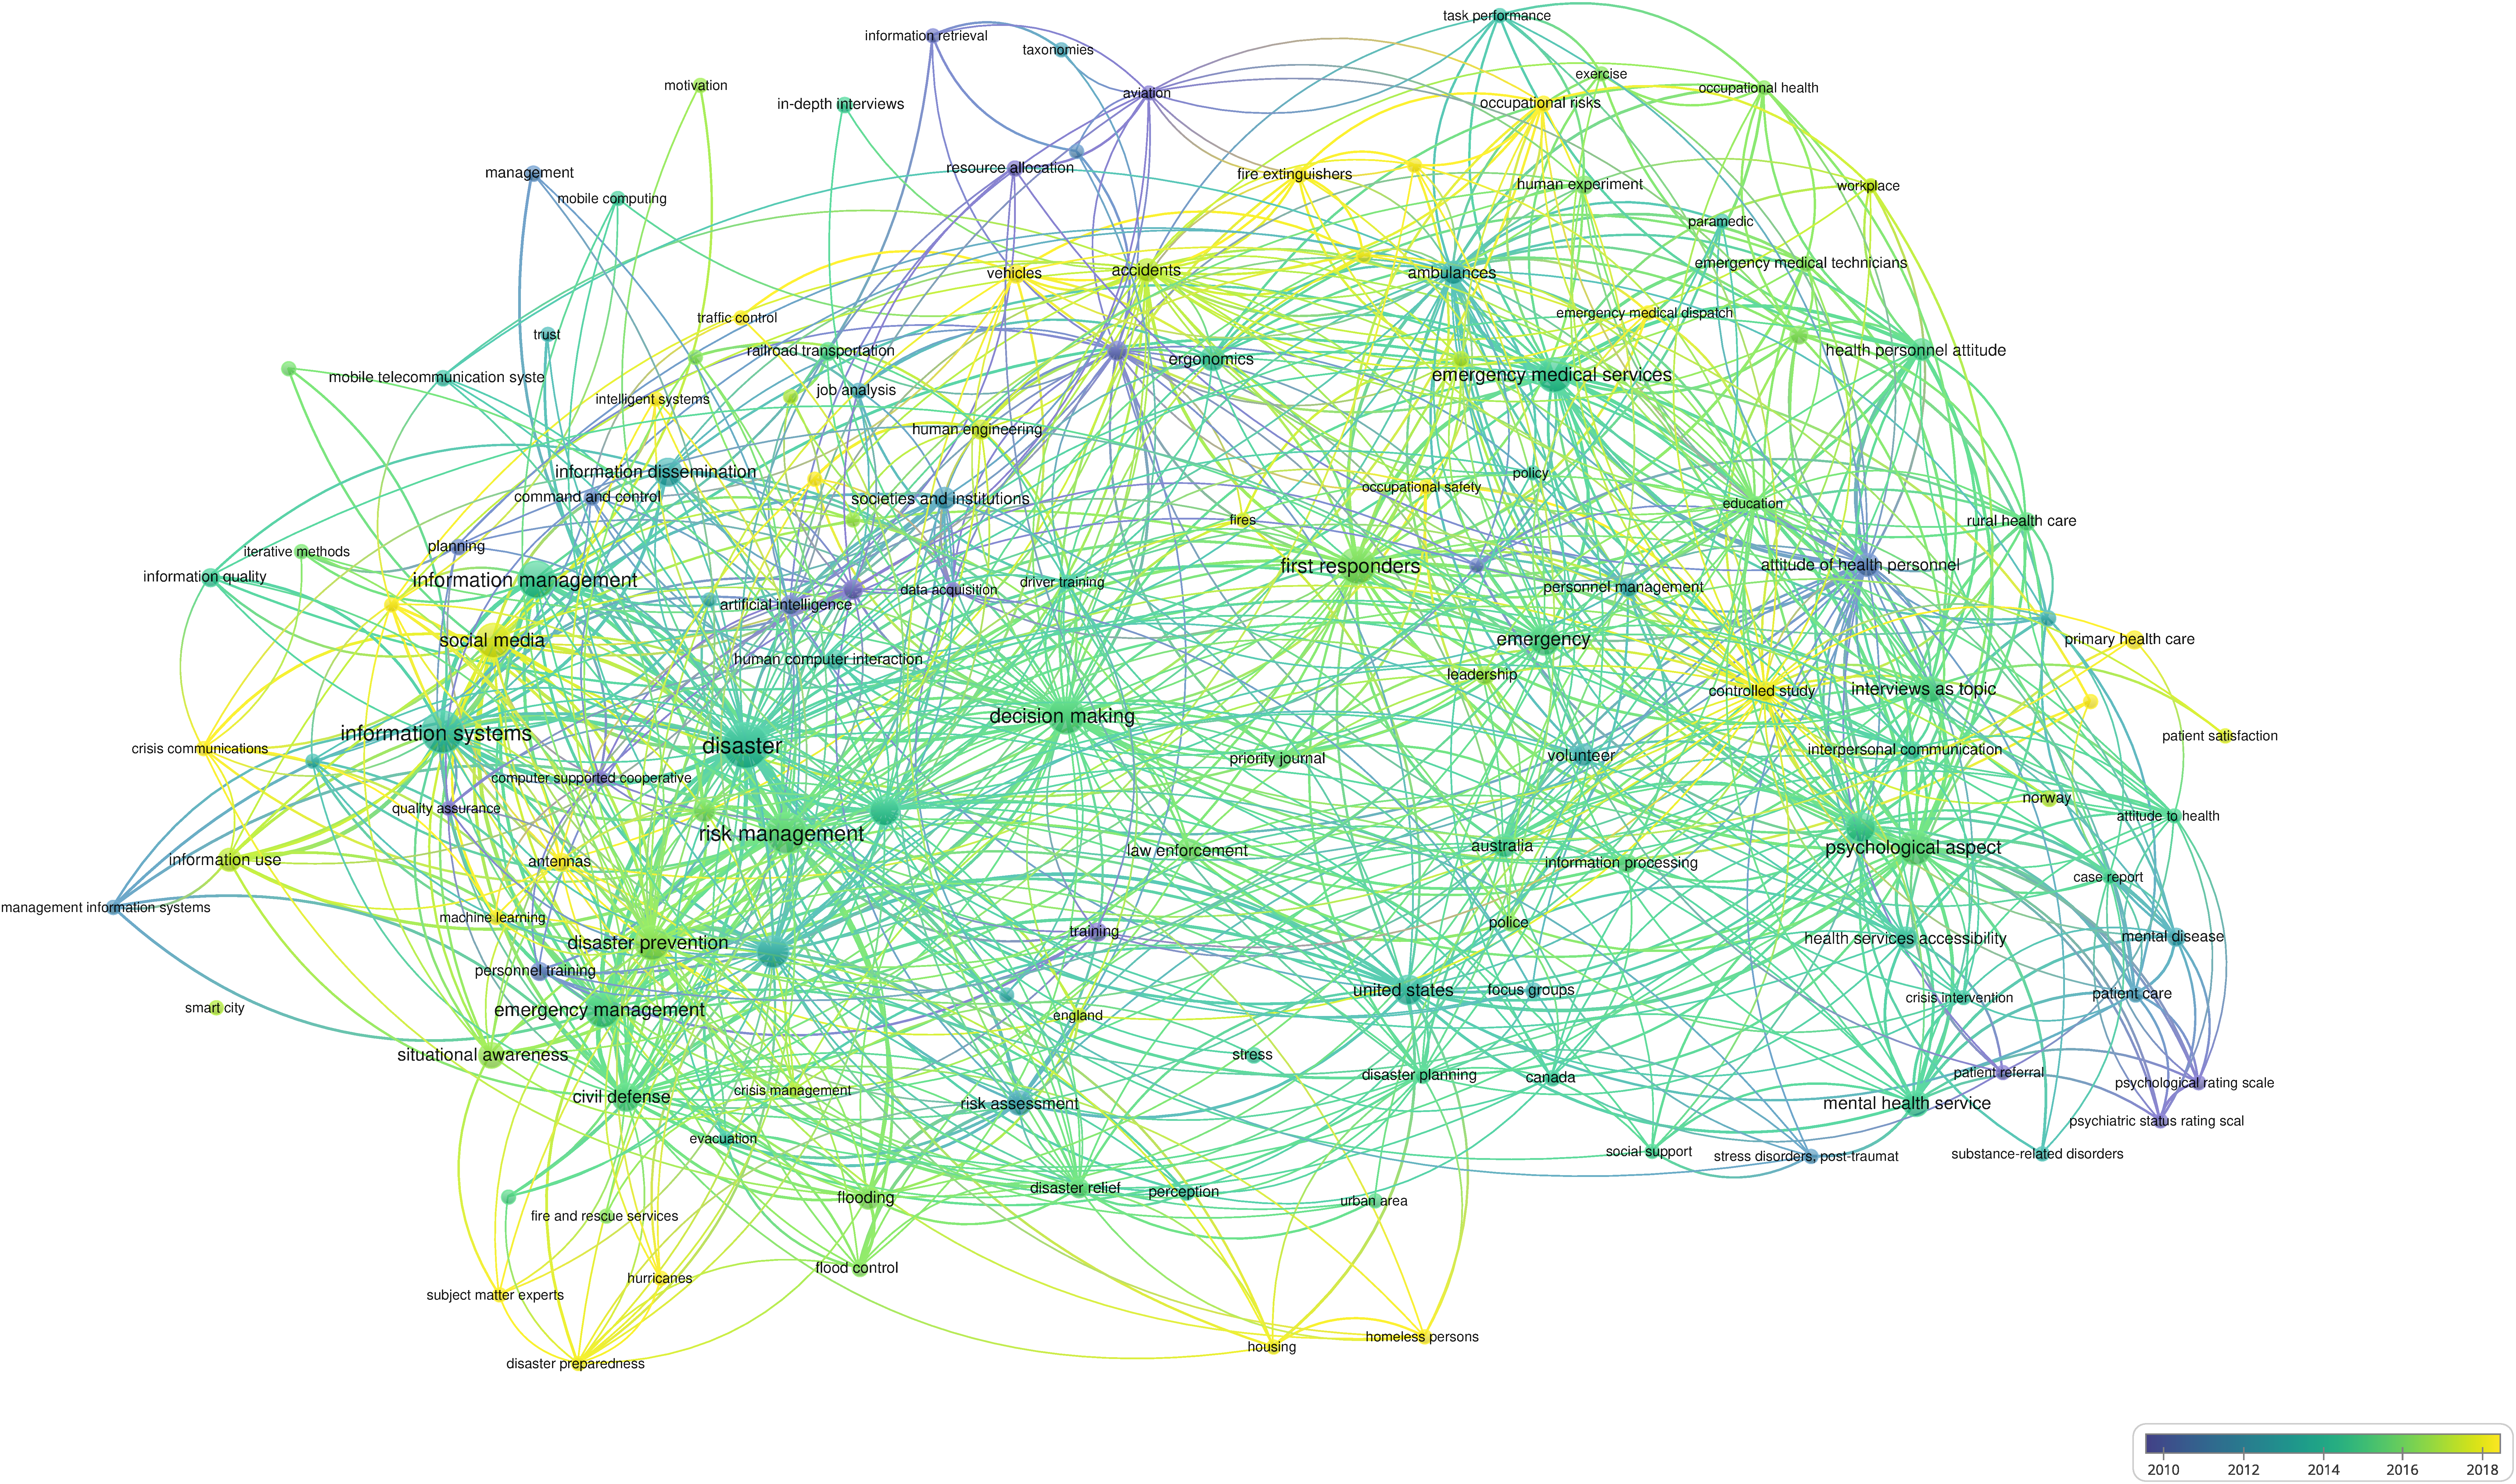
\includegraphics[width=\paperwidth,height=\paperheight,keepaspectratio]{figures/chap-2/business-needs-overlay.pdf}
        \caption{Distribution of keywords with more than 3 occurrences among the articles from the query on information needs of crisis responders.}
        \label{literature:business-needs-overlay}
    \end{figure}
\end{landscape}

The left cluster is composed of the most common keywords used in the fetched articles.
Keywords such as \emph{disaster}, \emph{information systems} and \emph{risk management} (Figure~\ref{literature:business-needs-bar}) are the most prominent ones and seems to be mostly used circa 2014.
Prior to that period (between 2010 and 2014), the field was mostly focusing on planification of resources and training.
But the field took a shift towards data processing to support \emph{decision making} during emergency events.
The collision with the other domains explored in this chapter seems to happen around 2018, were keywords such as \emph{machine learning}, \emph{social media} or \emph{situational awareness}.

\begin{figure}[htb]
    \centering
    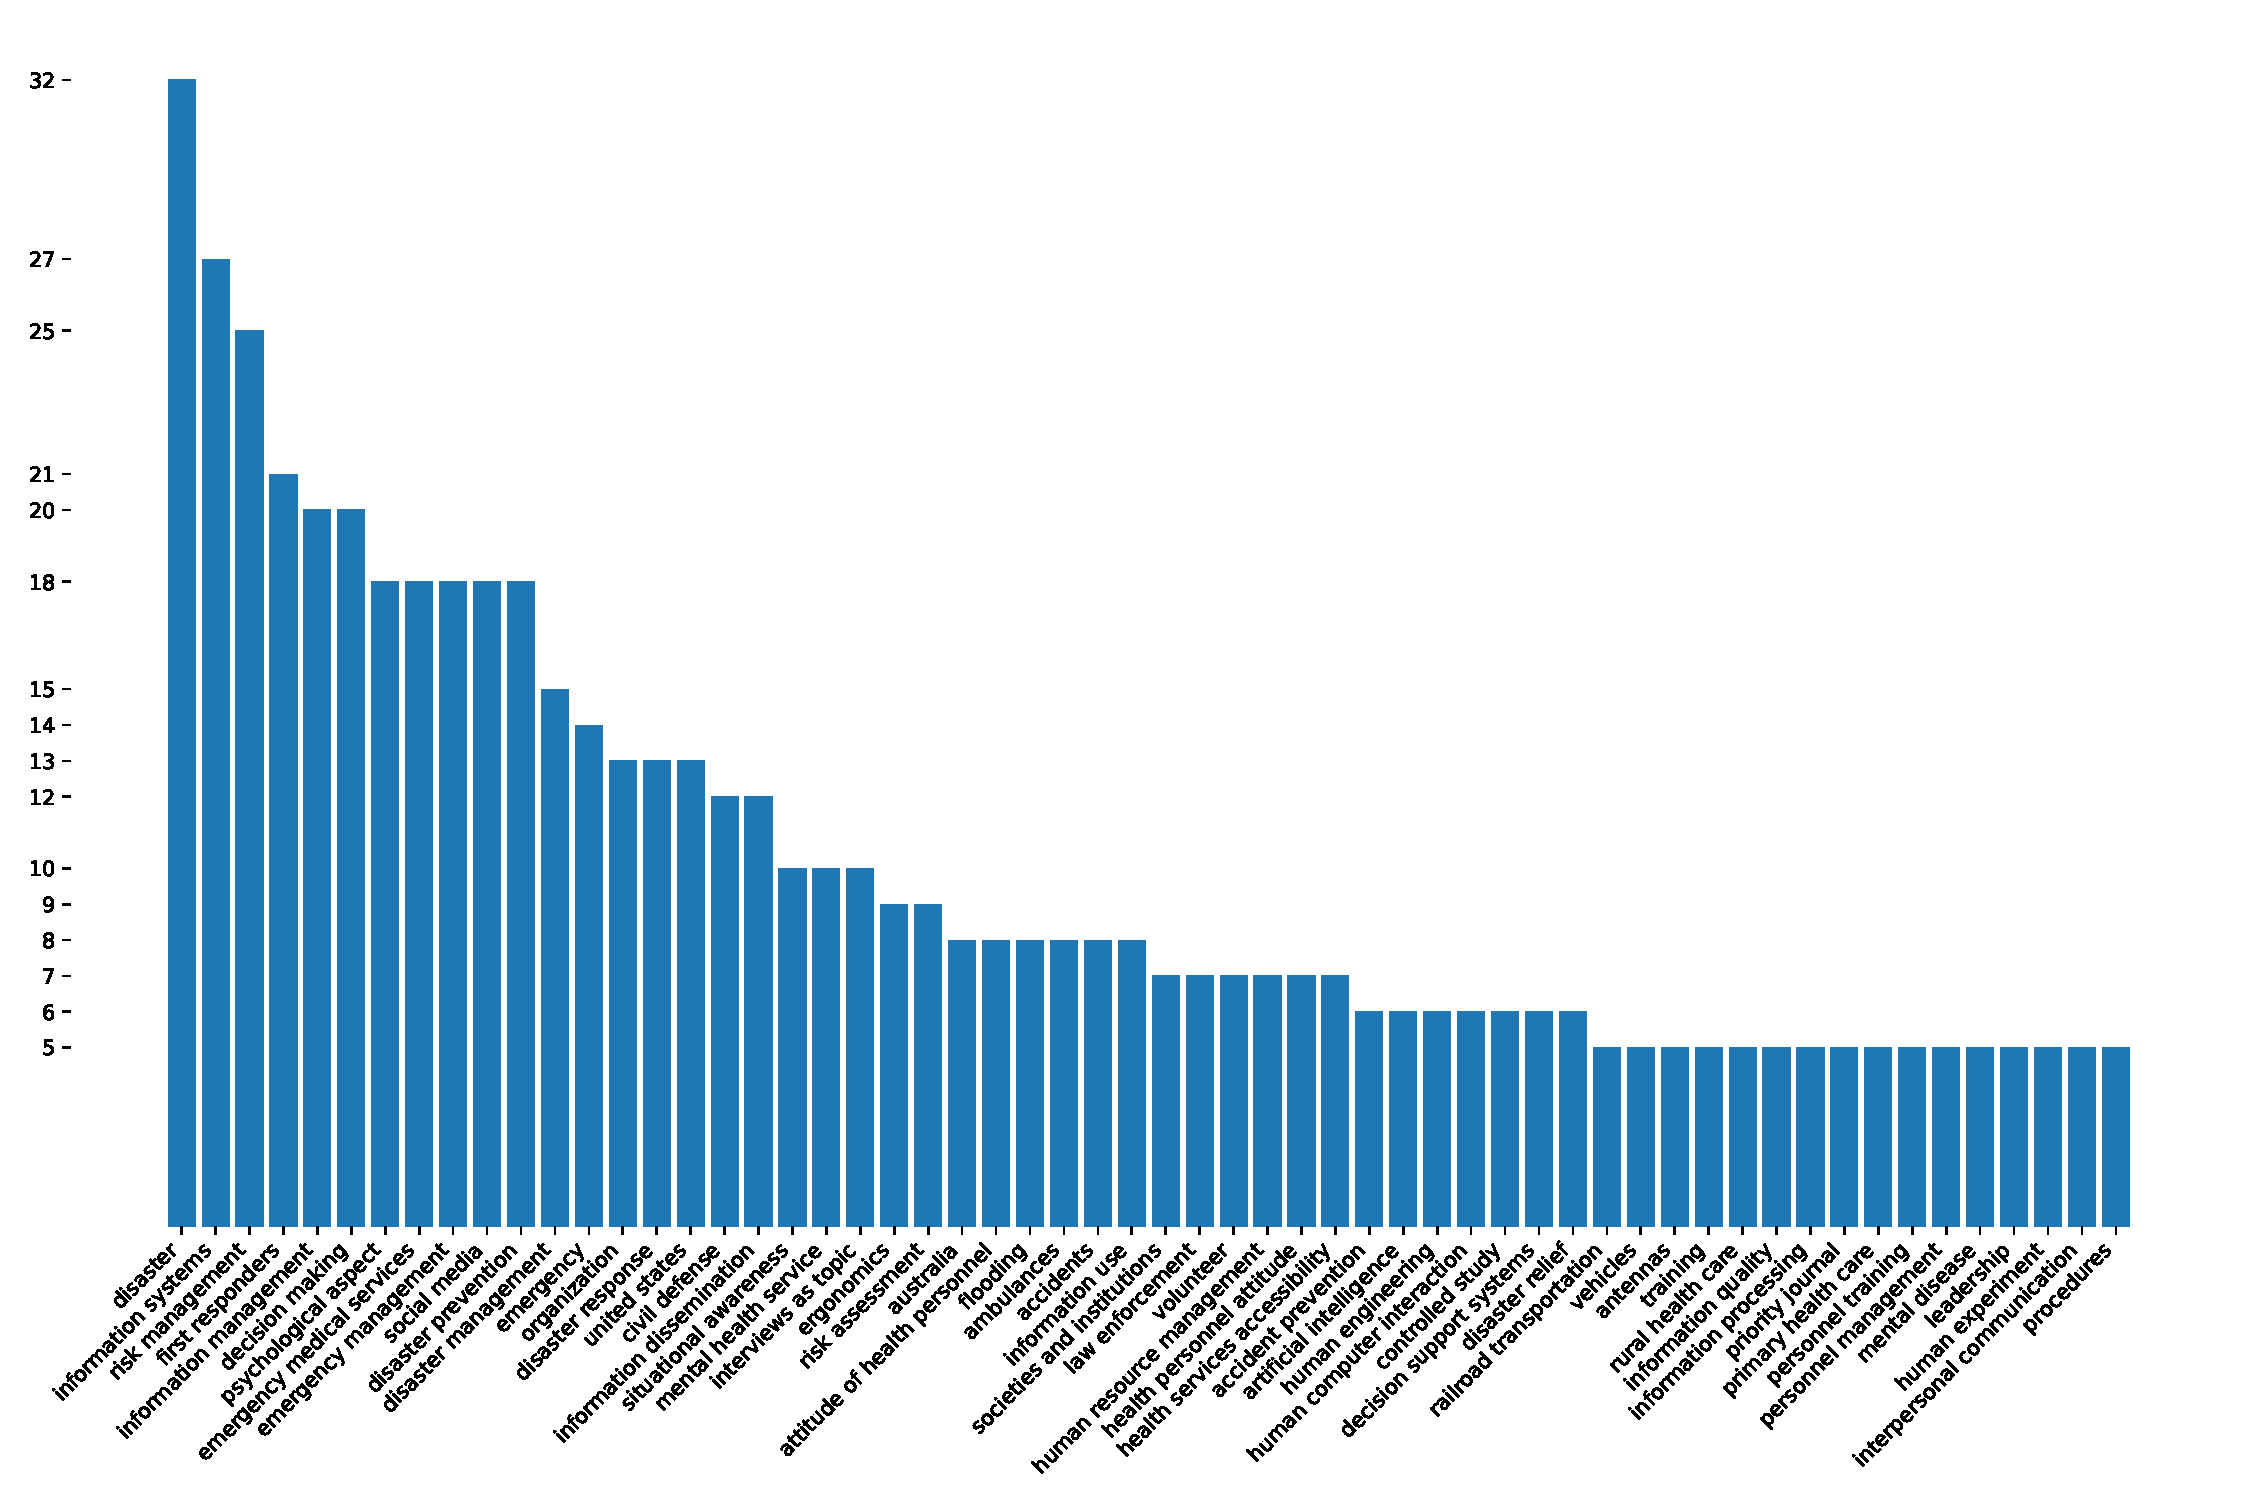
\includegraphics[width=\textwidth]{figures/chap-2/business-needs-bar.pdf}
    \caption{Distribution of keywords with more than 3 occurrences among the articles from the query on information needs of crisis responders.}
    \label{literature:business-needs-bar}
\end{figure}

Table~\ref{table:business-needs-main-articles} provides a summary of the responders need identified in the most prominent articles in the field.
Articles were selected if they had at least 25 citations, have been published in 2010 or after, are located in the information systems cluster and are not duplicates.
The articles retrieved provide insights on what are some of the pain points of emergency organizations.

Some studies are event specific, due to a governemental request or a gap in the emergency preparation cover.
\textcite{lindellTsunamiPreparednessOregon2010} is interested in tsunamis management on the US east coast and \textcite{cabreraaguileraModellingPerformanceVariabilities2016} tackle oil spill.
Both studies do not address any particular point in the management of this type of event.
Rather, they implement the entire crisis management cycle for these events, which were not considered until their work.
Unfortunately, no specific information need for decision-makers emerges.

On the other hand, others articles are most focused on specific needs of emergency organizations.
Collaboration, information sharing and joint preparation exercices are one of the concerns raised \parencite{berlinWhyCollaborationMinimised2011,parkerSurfaceWaterFlood2011}.
The increasing complexity of crisis events ask for a wider range of skills.
As no organization can possess all the required skills at the same time, other actors have to be involved.
Crisis management organization acknowledge that an unexpected collaboration between actors yield poor outcomes during the response.
Thus, exercices and discussions are key during the preparation phase and an adequate means of communication between the actors during the response are needs identified by the studies.

\textcite{yangDesignPrinciplesIntegrated2012} highlight an interesting and well mentioned need for crisis response: situation awareness.
Situation awareness correspond to the representation of the state of the environment that surround the emergency response organization during an event.
This representation directly guides decision making.
Consequently, building the best and most accurate representation possible directly at the start of the event is critical.
In there are articles, \citeauthor{yangDesignPrinciplesIntegrated2012} emphasize 4 critical pieces of information for situational awareness:

\begin{enumerate}
    \item Environmental conditions such as the building infrastructure, number of occupants, and the exact location of any hazard;
    \item Information on the response participants such as who is involved in the response, what skills they could offer, and what resources they bring to the scene;
    \item The status of any casualties, the accident location, cause, and severity; and
    \item The available resources including equipment and food.
\end{enumerate}

As per the authors, "timeliness, accuracy, and completeness are the critical dynamic attributes of these four categories of information".
The next chapter (chapter 3) will dive deeper into this concept.

The issue with building an accurate situation awareness is the need for information.
With the disruption of the regular means of communication and information channels, decison makers are shrouded in darkness.
According to \textcite{tapiaTrustworthyTweetDeeper2013,cobbDesigningDelugeUnderstanding2014}, some emergency centers acknowledge the benefit of social media as a potential information source.
However, the issue identified is the lack of tools and methods, similar to the ones that built for calls, for social media.

Finally, the last need identified among the extracted items is the communication to the public.
\textcite{aloudatRegulationUbiquitousMobile2011} insist on the potential yielded by modern communication means such as cell phones and social media to share information with the public during an event.
As people are not always around a radio or a TV, they often miss critical messages during fast moving events (floods, fires...), resulting in casualties.
On the other hand, (almost literally) most of the population carry a cellphone nowadays, and the critical messages could be distributed faster and with a better viewing rate than traditional methods.
Text messages or notifications from social media could be more effective communication channels that emergency response teams should use.

\begin{table}[bp]
    \centering
    \renewcommand{\arraystretch}{1.5}
    \caption{Articles on informational needs of emergency responders retrieved from the previous request with at least 25 citations.}
    \begin{tabular}{m{0.25\textwidth} m{0.75\textwidth}}
        Reference                                                   & Business need identified by the authors.                                                                                                                                                                               \\ [0.5ex]
        \toprule
        \cite{lindellTsunamiPreparednessOregon2010}                 & Tsunami training                                                                                                                                                                                                       \\
        \cite{aloudatRegulationUbiquitousMobile2011}                & Communication to the public                                                                                                                                                                                            \\
        \cite{berlinWhyCollaborationMinimised2011}                  & Collaboration between the different actors                                                                                                                                                                             \\
        \cite{parkerSurfaceWaterFlood2011}                          & Create conversations between unusual actors during the preparation phase                                                                                                                                               \\
        \cite{yangDesignPrinciplesIntegrated2012}                   & Increase situation awareness, Identify key informations~\footnote{(hazard environment, information concerning the responder workforce, information on evolving safety issues, and information about safety equipment)} \\
        \cite{tapiaTrustworthyTweetDeeper2013}                      & Accounting for informal sources of data (such as social media)                                                                                                                                                         \\
        \cite{cobbDesigningDelugeUnderstanding2014}                 & Big data processing methods adapted to social media data                                                                                                                                                               \\
        \cite{cabreraaguileraModellingPerformanceVariabilities2016} & Oil spill preparation                                                                                                                                                                                                  \\
        \bottomrule
    \end{tabular}
    \label{table:business-needs-main-articles}
\end{table}

\subsection{Information gathering: place of social media?}
Looking back at the first chapter, the sub problematic linked to this section was: \emph{What information that can be obtained from social media is relevant to the decisiom makers in crisis response?}
The two previous subsections identified several references that explored the pain points of decision makers in crisis management.
Each sub-section respectively explored top-down and bottom-up approaches to crisis management understanding.
However, social media were not directly considered in the query made on the bibliographic database as social media are not the only concern of these fields.

This sub-section emphasize on the intersection of the previous results and social media.
Crisis situation models:
Among the 205 documents on crisis situation models, 22 articles include the keywords \emph{social media} or \emph{twitter} to the query.
Two articles from the list of articles qualified as prominent are centered on social media:

\begin{itemize}
    \item \textcite{purohitIdentifyingSeekersSuppliers2014}
    \item \textcite{ghahremanlouGeotaggingTwitterMessages2014}
\end{itemize}

The same approach applied to the needs of crisis management organizations provides a similar number of articles.
22 articles among the 219 mention \emph{social media} or \emph{twitter}.
Among the articles studied in the previous part, two are dedicated to social media:

\begin{itemize}
    \item \textcite{cobbDesigningDelugeUnderstanding2014}
    \item \textcite{tapiaTrustworthyTweetDeeper2013}
\end{itemize}

In both cases, only roughly 10\% of the total body of surveys mention social media.
% From the remaining articles, most of the ontologies or metamodels are studied and represent information flows during an event.
% For instance, \textcite{montarnalAutomatedEmergenceCrisis2017} create an ontology to merge data coming from social media and sensors.
% \textcite{gaurEmpathiOntologyEmergency2019} followed up by adding satellites images.
% It appears that the information available during the event and the management of the same event are too different to get associated in the same representation.
% Despite this explanation, very few link the two to create a representation of emergency management mindful of the information available.

\subsection*{Conclusion}
This section was answering the question: \emph{what is the decision-making context in emergency situations?}
This issue has attracted a fair amount of attention and this section explored two ways taken by two research communities to answer this question.
These two ways correspond to the two subsections.
The first sub-section was dedicated to model engineering and the previous attempts to create representations
or abstractions to represent the concepts involved in an emergency.
This approach is fed by the need of automation of certain tasks in crisis management, hence the need of concepts to represent and manage the different aspects.
However, this approach is essentially top-down, and few references report feedbacks from field interviews.

This insight feeds the need to gather the information requirements of the primary users during their operations.
Hence, the second sub-section, dedicated to the report of the problems that crisis management organizations face, gathered through interviews.
Yet, this bottom-up approach produces unstructured results, which cannot be directly translated with an automatic

Overall, the needs identified to improve crisis management from both approaches outcomes are:

\begin{itemize}
    \item Situation Awareness
    \item Collaboration
    \item Communication to the public
    \item Social media accounting
    \item Sensor data integration
    \item Large data volume processing
\end{itemize}

The next section will be dedicated to the existing means of identifying and mining information from social media.

\section{NLP tools for information extraction from social media data}
The first chapter presented the NLP domain.
Through the development of this domain, many tools, algorithms and methods have been developed to process textual data.
With the emergence of social media, a new source of textual data appeared, and with it, its own challenges.

This sections tackles the sub problematic: \emph{How can these information be obtained, in the context of crisis informatic?}
Social media data are used as a data source in a various of use cases.
This section is broken down into two parts and it aims to explore two directions.
First, for which applications natural language processing is used on social media data?
Secondly, how are these information extracted?
Each direction has its own dedicated sub-section.

To explored these two direction the following request is run:

\begin{itemize}
    \item (TITLE-ABS-KEY({natural language processing} or {information mining}))
    \item AND (TITLE-ABS-KEY({social media} or Twitter))
    \item AND (TITLE-ABS-KEY(survey))
    \item AND (EXCLUDE(DOCTYPE, "re") OR EXCLUDE(DOCTYPE, "cr"))
\end{itemize}

The idea behind this request is as follow:

\begin{itemize}
    \item Use "natural language processing" or "information mining" as a keyword.
    \item In addition to the previous ones, they also have to include "social media" or "twitter".
    \item This request only retrieve surveys.
    \item It excludes articles that present conference tracks and or reviews of other articles.
\end{itemize}

Contrary to other sections, this one wil take surveys as a proxy to study the domain.
Without the constraint put on surveys, the request returns 4231.
As this volume of publication could not be processed in a reasonable amount of time, the choice have been to look only at surveys.
However, this hypothesis seems reasonable, considering the fact that the goal is to identify the main trends in the field.

The request returns 217 surveys, published between 2011 and 2021 (Figure~\ref{literature:nlp-hist}).
The volume of documents fetched from this request is similar to the previous ones, despite looking only at surveys.
While being a fairly recent research venue, the interest for NLP uses on social media data is really high and increased over the years..

\begin{figure}[htb]
    \centering
    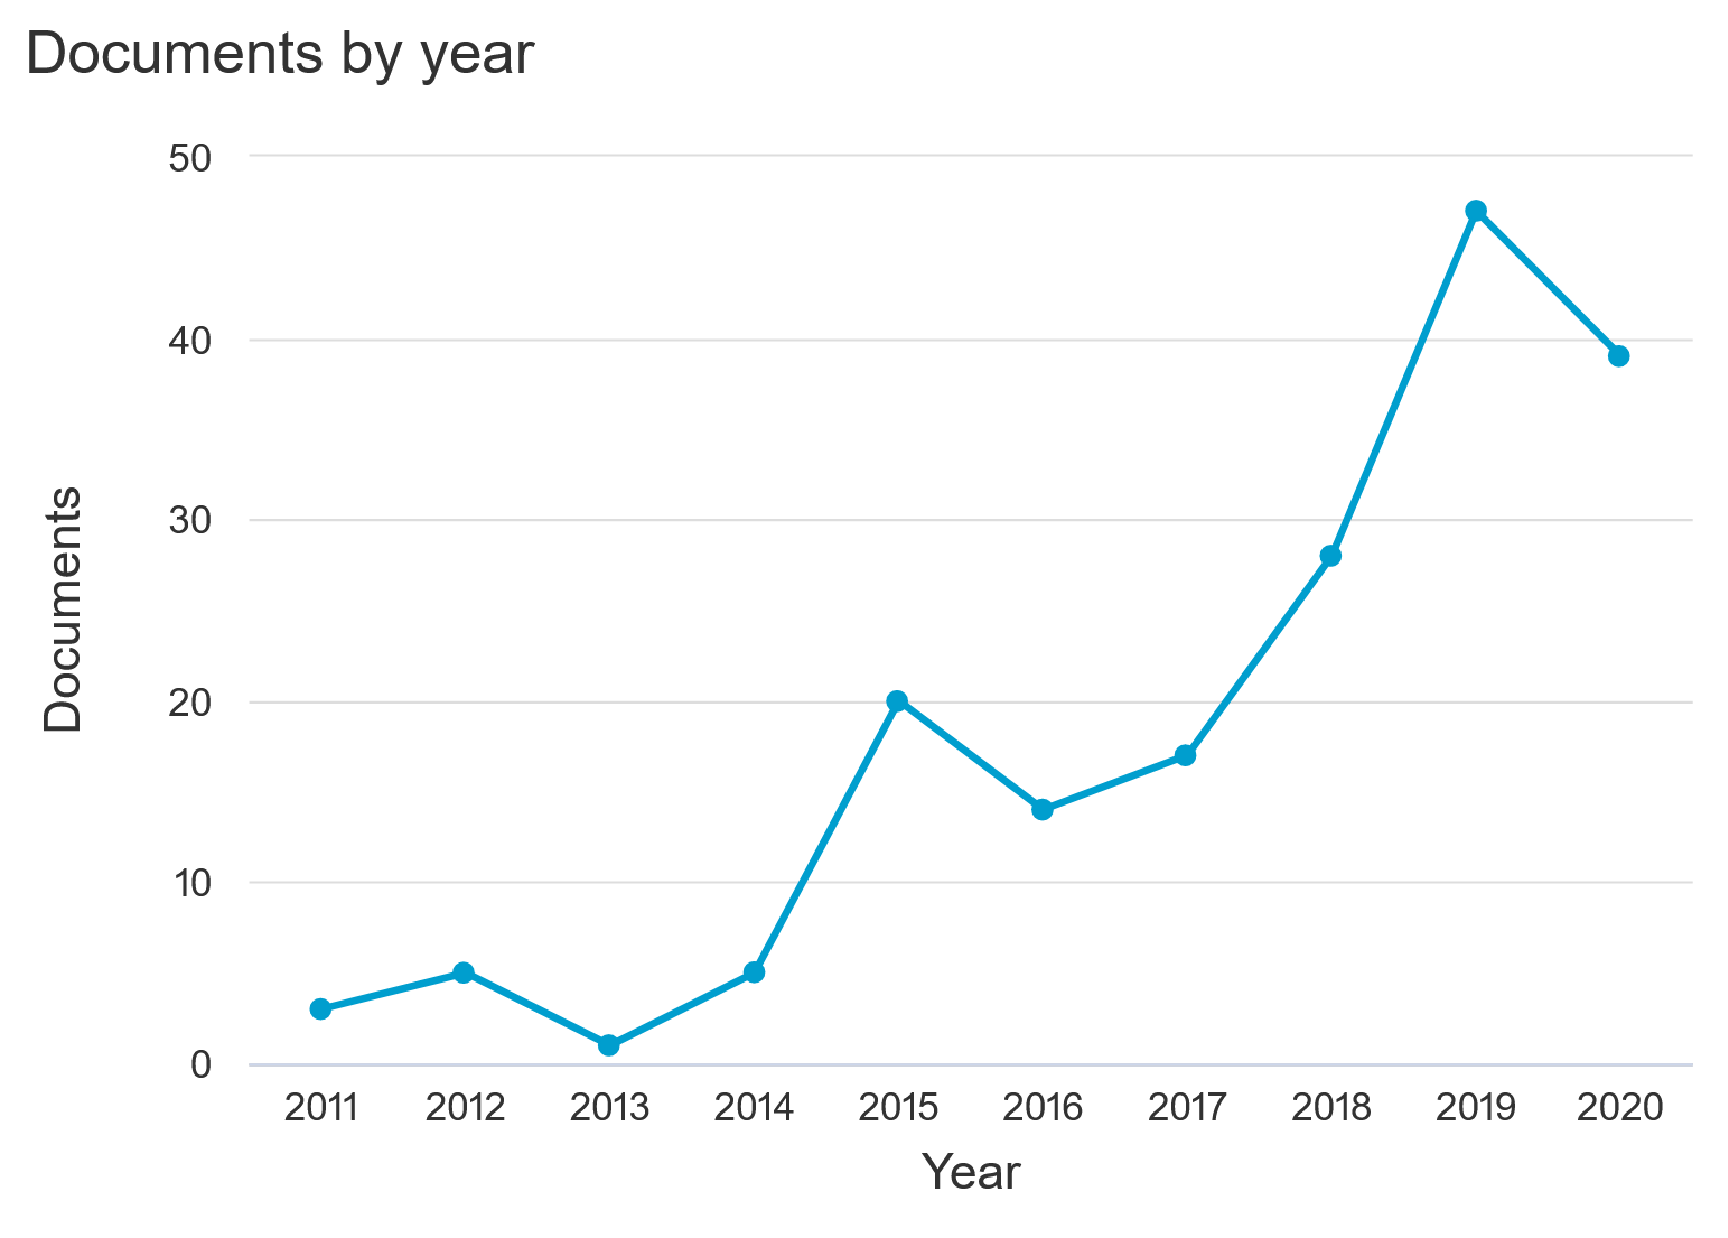
\includegraphics[width=\textwidth]{figures/chap-2/nlp-hist.pdf}
    \caption{Timelime of the volume of contributions per years for the application of NLP methods to social media data. The year 2021 is excluded because the year is not complete at the time of writing.}
    \label{literature:nlp-hist}
\end{figure}

The surveys retrieved appears as a single cluster (Figure~\ref{literature:nlp-overlay}).
This overlay was created by aggregating synonyms, removing the keywords from the query and some keywords with low value for our study ("state of the art, large amounts, codes (symbols), research questions, text").
Despite the youth of the field, its evolution is very fast, both in terms of applications and methods used.
Circa 2011, the field was essentially centered around epidemiological applications and statistical analyses.
From this point on, a kaleidoscope of applications and methods were used.
They are detailed in the next two subsections.

\begin{landscape}
    \begin{figure}[htb]
        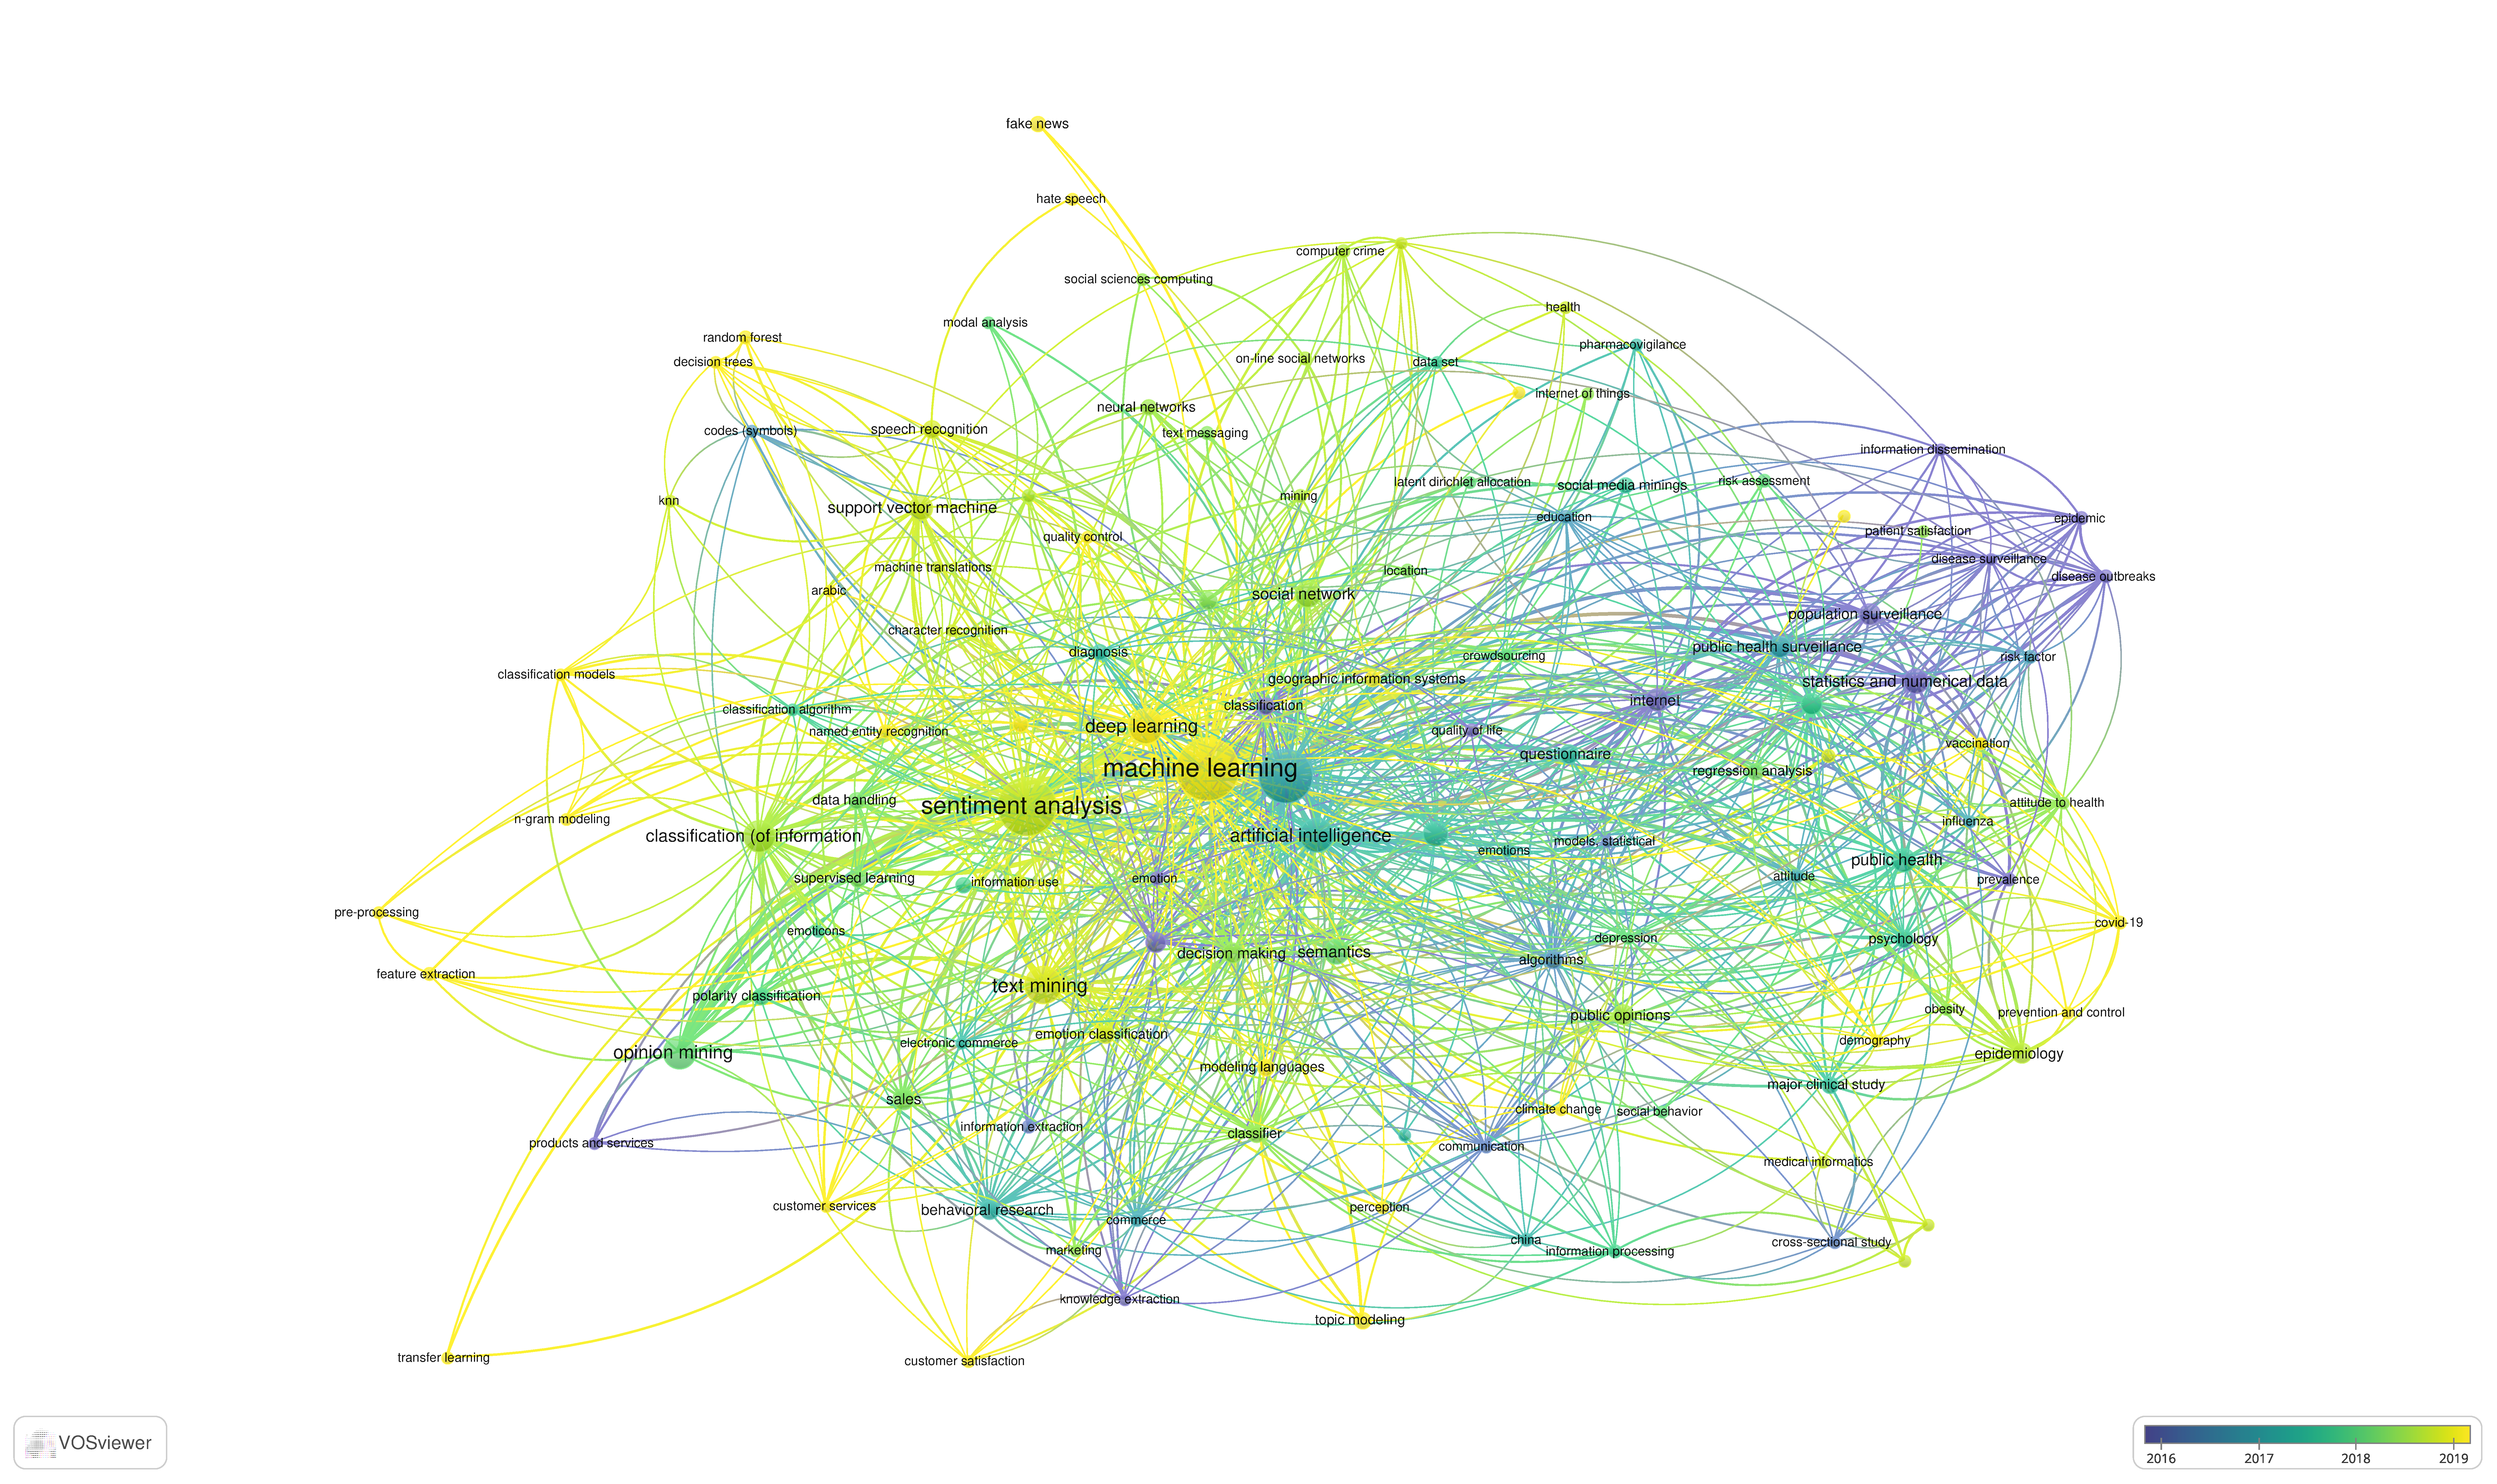
\includegraphics[width=\paperwidth,height=\paperheight,keepaspectratio]{figures/chap-2/nlp-overlay.pdf}
        \caption{Distribution of keywords with more than 3 occurrences among the articles from the query on NLP applied on social media data.}
        \label{literature:nlp-overlay}
    \end{figure}
\end{landscape}

However, form these years, some trend are more prominent than others.
On the application side, \emph{sentiment analyses} is by far the most studied application (73 mentions of this keyword) (Figure~\ref{literature:nlp-bar}).
Mining applications are second with \emph{data mining} (mentioned 61 times), \emph{text mining} (30 times) and \emph{opinion mining} (mentioned 21 times).
On the method side, \emph{artificial intelligence} (mentioned 25 times), and specially \emph{machine learning} (85 times, almost half surveys) methods (such as \emph{deep learning}) are heavily mentioned as well in the surveys.
This probably comes from the parallel advances made in NLP through the renew of machine learning.

\begin{figure}[htb]
    \centering
    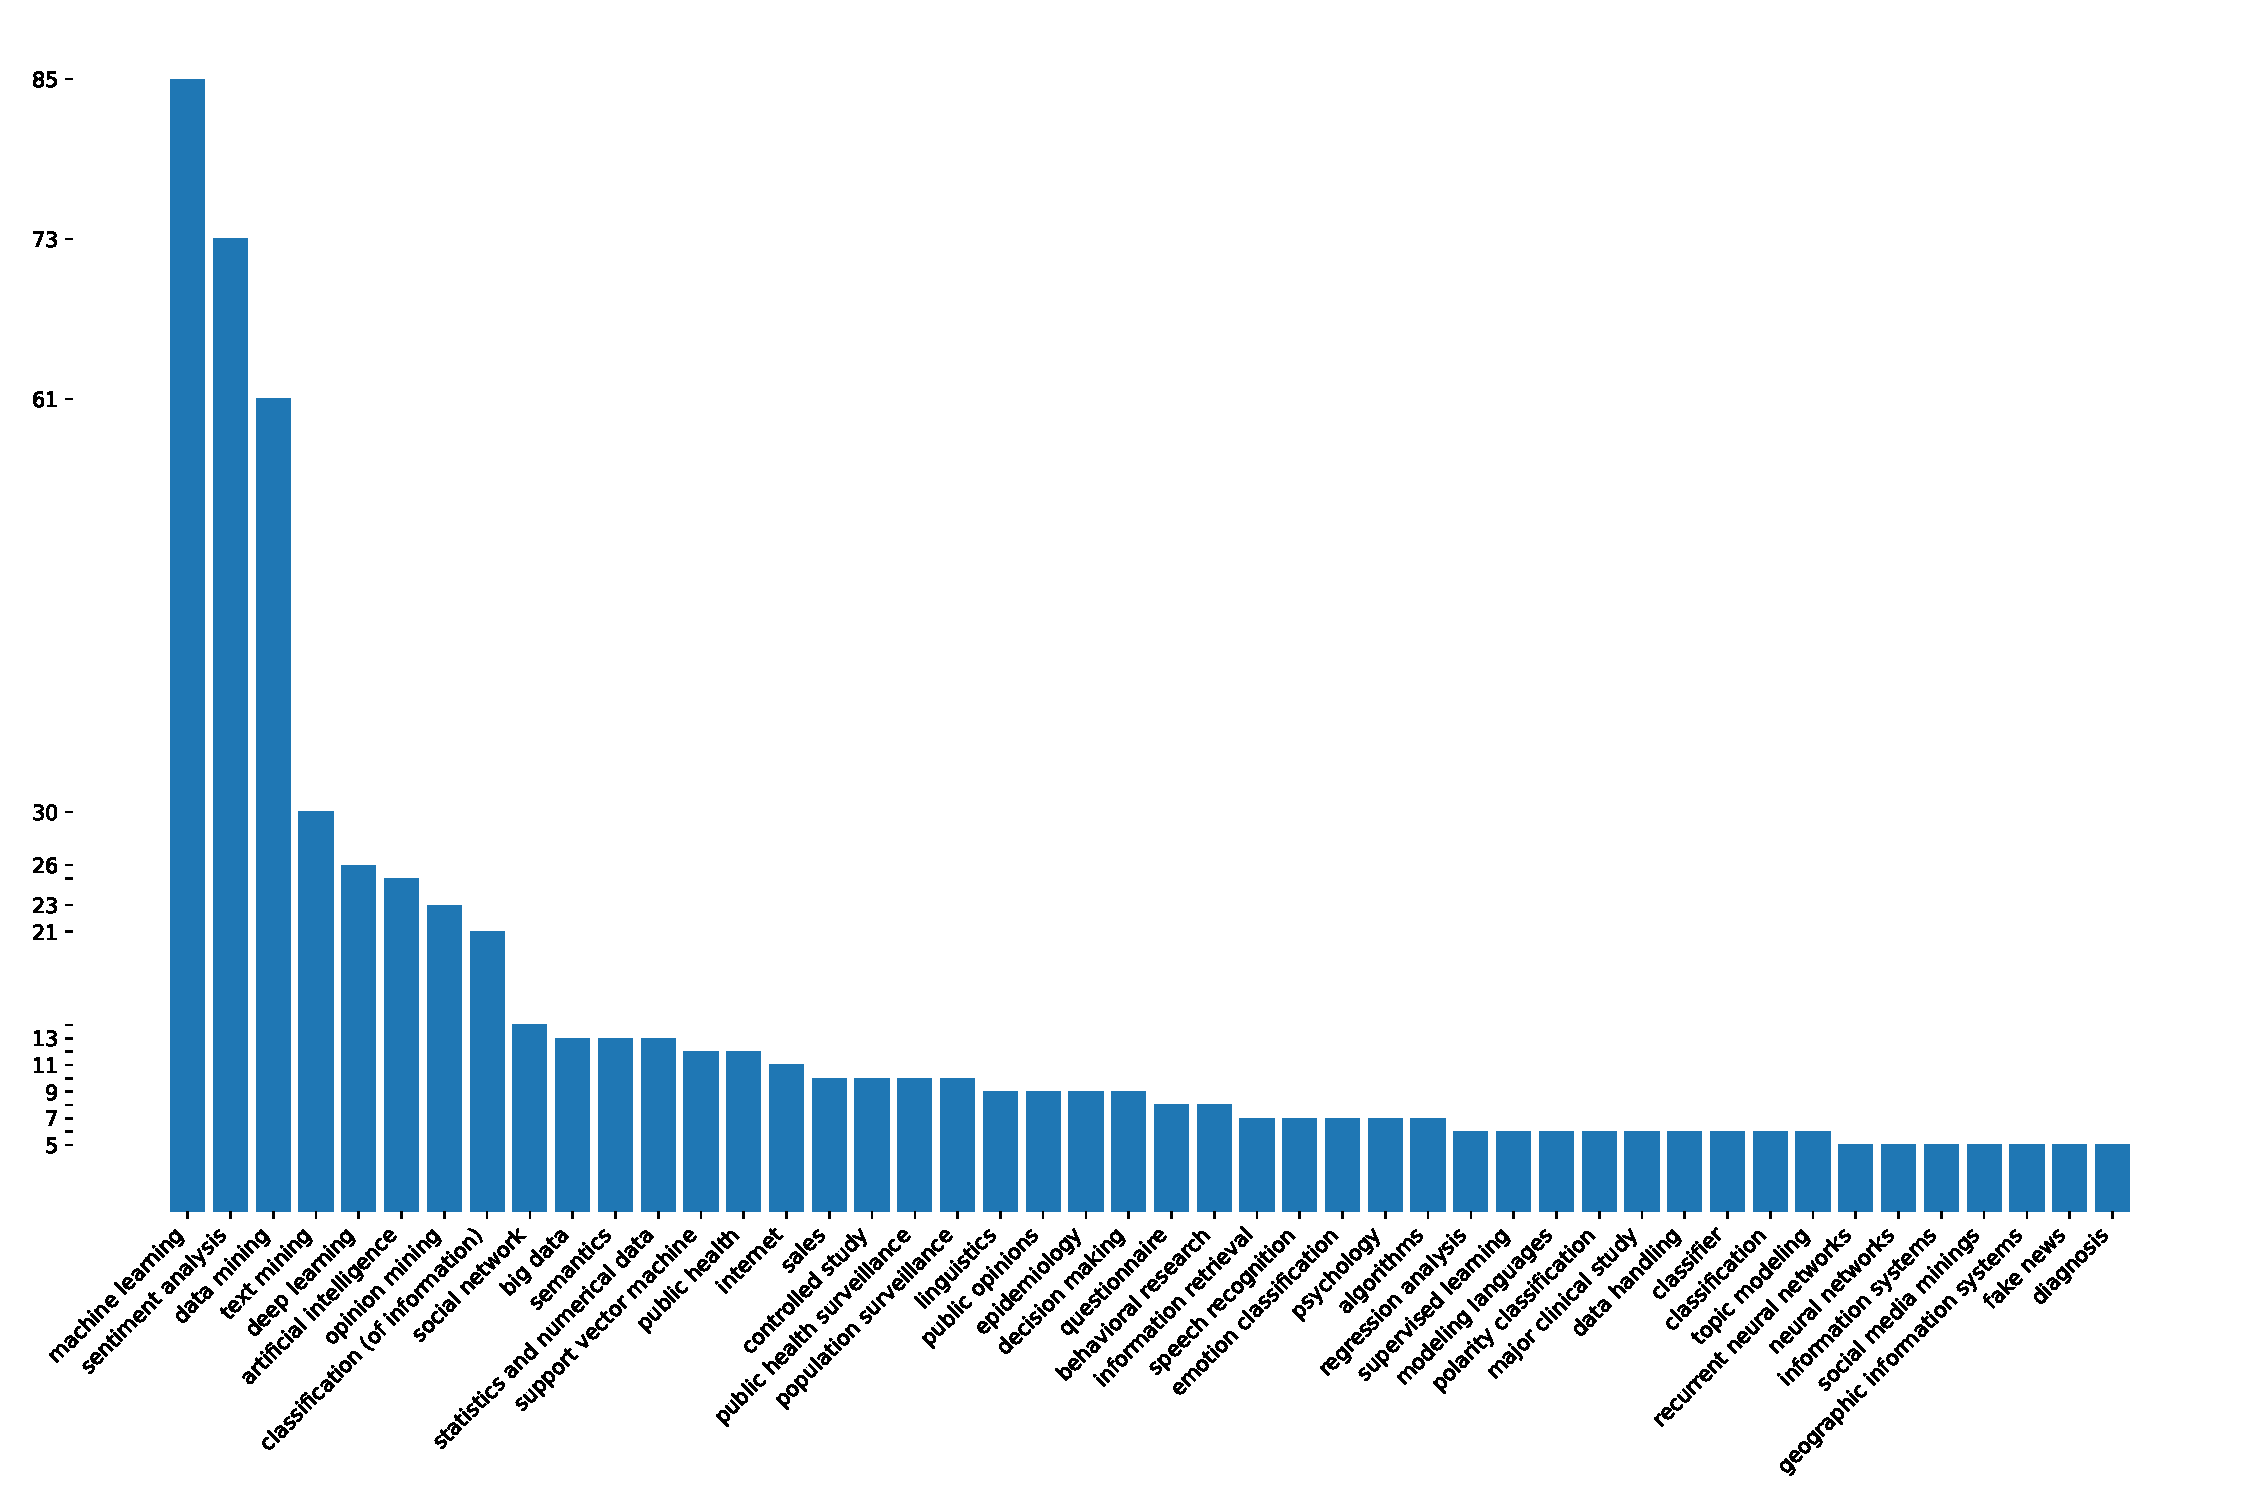
\includegraphics[width=\textwidth]{figures/chap-2/nlp-bar.pdf}
    \caption{Distribution of keywords with more than 4 occurrences among the articles from the query on NLP applied on social media data.}
    \label{literature:nlp-bar}
\end{figure}

The next sub-section explores the application mentioned by the surveys obtained from the request.

\subsection{Social media information extracted using NLP}
Social media data contain valuable information for a wide range of applications.
The surveys fetched contains several application domains in their keywords.
They are summarized in Table~\ref{table:application-domains}.
Some of the keywords are grouped to reflect the major domain they depend on.
Also, some keywords were common to multiple topics.
For instance, \emph{attitude} is used both in health and business related surveys.
\emph{quality of life} is used in urban issues, breast cancers, depression detection and opioids side effects.
Other keywords that did not belong to any major category have been grouped in a separated category.

Thus, there are seven major domains identified:

\begin{itemize}
    \item Epidemiology
    \item Medical Informatic
    \item Behavioral Research
    \item Social Media Research
    \item Business
    \item Information Science
    \item NLP Challenges
\end{itemize}

NLP applied to social media is used for a variety of medical applications.
Epidemiology, which study the distribution and frequency of diseases as everyone knows by now,
is interested in social media to monitore the mention of symptoms by users in order to detect and observe the spread of a disease.
This include, of course, the COVID-19 outbreak or the influenza outbreak in (2009-2010).
Broader medical applications are labeled under "Medical Informatic".
It contains applications using the same methodology, but applied to other diseases or conditions, such as \emph{depression}, \emph{obesity} or \emph{pregnancy}.
Social media are also considered for \emph{pharmacovigilance} to monitore secondary effets (\emph{patient satisfaction}, \emph{opiate addiction}).
The behavior of the urban population (\emph{smartcity}, \emph{computer crime}) or society in general (\emph{demography}, \emph{population surveillance}) can also be observed through social media.
Their expressed feelings towards events or political decisions can then be quantified and analyzed.
Social medias, as digital twins of society, are also environments that bring some reflections of its own.
The phenomenon of \emph{fake news} in particular has taken many actors in society by surprise and is an issue that attracts a lot of attention.
The way in which information spreads within the \emph{social network} of users or its very structure, are also topics of research.
Marketing departments and PR firms are also naturally very interested in the insights available on social media.
The management of the content of social media and specially the \emph{information extraction} and \emph{knowledge extraction} part
are challenges for the information science domain.
Social media data also come with their own challenges for the NLP domain.
Social media content is noisy, informal and often come with its own use of the grammar.
Consequently, most of the methods applied on other text are disrupted with social media data.
\emph{machine translation}, \emph{named entity recognition} and other tasks are then explored and improved in this context.
Alongside improvements on several tasks, social media are also widely used to \emph{sentiment analysis}, \emph{topic modeling} or \emph{polarity classification}.
In the final catergory, interesting topics appear such as \emph{crowdsourcing}.
Indeed, some sociologists, instead of exploiting social media, leverage their power to achieve goals, and then study mechanisms that can encourage positive actions for instance.
Of course, \emph{climate change} is also an application mentioned, considering the importance of this topic.

\begin{center}
    \begin{longtable}{ rl }
        \caption{Applications domains}                            \\
        Major domain            & Sub domains                     \\
        \bottomrule
        Epidemiology            & COVID-19                        \\
                                & disease outbreaks               \\
                                & disease surveillance            \\
                                & vaccination                     \\
                                & epidemic                        \\
                                & epidemiology                    \\
                                & influenza                       \\
        Medical Informatic      & depression                      \\
                                & diagnosis                       \\
                                & psychology                      \\
                                & public health surveillances     \\
                                & health survey                   \\
                                & risk factor                     \\
                                & major clinical study            \\
                                & medical informatics             \\
                                & obesity                         \\
                                & opiate addiction                \\
                                & opioid-related disorders        \\
                                & patient satisfaction            \\
                                & pharmacovigilance               \\
                                & pregnancy                       \\
                                & prevalence                      \\
                                & prevention and control          \\
                                & quality control                 \\
                                & risk assessment                 \\
                                & controlled study                \\
        Behavioral Researches   & social behavior                 \\
                                & models, statistical             \\
                                & computer crime                  \\
                                & public opinion                  \\
                                & population surveillance         \\
                                & demography                      \\
                                & smart city                      \\
                                & risk assessment                 \\
        Social Media Researches & facebook                        \\
                                & social media mining             \\
                                & social network                  \\
                                & fake news                       \\
                                & modal analysis                  \\
                                & data mining                     \\
                                & information dissemination       \\
                                & opinion mining                  \\
                                & perception                      \\
        Business                & commerce                        \\
                                & customer services               \\
                                & sales                           \\
                                & communication                   \\
                                & electronic commerce             \\
                                & marketing                       \\
                                & products and services           \\
        Information Science     & knowledge extraction            \\
                                & information systems             \\
                                & classification (of information) \\
                                & gis                             \\
                                & decision making                 \\
                                & information extraction          \\
                                & information processing          \\
        NLP challenges          & machine translations            \\
                                & speech recognition              \\
                                & polarity classification         \\
                                & location inference              \\
                                & text mining                     \\
                                & automated detection             \\
                                & named entity recognition        \\
                                & arabic languages                \\
                                & linguistics                     \\
                                & topic modeling                  \\
                                & emotion analysis                \\
                                & sentiment analysis              \\
                                & emoticons                       \\
                                & modeling languages              \\
        No specific category    & china                           \\
                                & education                       \\
                                & crowdsourcing                   \\
                                & climate change                  \\
                                & quality of life                 \\
                                & attitude                        \\
                                & internet of things              \\
                                & spatiotemporal analysis         \\
                                & surveys and questionnaires      \\
        \bottomrule
        \label{table:application-domains}
    \end{longtable}
\end{center}

\subsection{NLP's tools to process previous data}
The previous sub-section presented the different applications of NLP on social media data.
The surveys retrieved also mentioned algorithms, methods or models related to NLP.
This sub-section aims to briefly present the different methods mentioned.
Table~\ref{table:nlp-tools} shows the keywords used in the surveys and groups them according to the different fields of artificial intelligence to which they belong.

\begin{table}[bp]
    \centering
    \caption{Main NLP algorithms and techniques that appear among the keywords}
    \begin{tabular}{rl}
        High level category     & Keywords used in the surveys  \\
        \toprule
        Data management         & Big Data                      \\
                                & Pre-processing                \\
                                & Feature Extraction            \\
                                & N-gram Modeling               \\
        Artificial intelligence & Artificial Intelligence       \\
                                & Algorithms                    \\
                                & K-Nearest Neighbors           \\
        Machine learning        & Statistical Model             \\
                                & Regression Analysis           \\
                                & Classification Algorithms     \\
                                & Classifiers                   \\
                                & Supervised Learning           \\
                                & Decision Trees                \\
                                & Random Forests                \\
                                & Support Vector Machine        \\
                                & Latent Dirichlet Allocation   \\
        Deep learning           & Neural Networks               \\
                                & Classification Models         \\
                                & Convolutional Neural Networks \\
                                & Recurrent Neural Networks     \\
                                & Transfer Learning             \\
        \bottomrule
    \end{tabular}
    \label{table:nlp-tools}
\end{table}

The many applications above require many different algorithms, capable of meeting different needs.
As already mentioned, data from social media are particular compared to the usual corpus composed of books and national newspapers.
This particularity, combined with the specificities of textual data, can be found through keywords such as \emph{Pre-processing}, \emph{feature extraction} or \emph{N-gram modeling}.
Pre-processing refers to the different steps that clean/prepare the data before they are passed to the algorithm.
N-gram modeling is one of the possible step and consists in grouping the tokens of a sentence into groups of N tokens.

The data are then provided to the processing algorithms.
Most of the algorithms mentioned in the survey are machine learning algorithms.
These algorithms build \emph{statistical models} based on distribution of tokens in sentences to provide results.
There are different categories of algorithms for different use cases.
\emph{Classification algorithms} are algorithms designed to assign data to a category.
On the other hand, \emph{regression} algorithms provide a value in a numerical range.
These models can be either \emph{classifiers} or regression models.
Most of these models are \emph{supervised} meaning that they require a dataset where all the data are annotated with a label.
Models can also be semi-supervised (only a portion is annotated) or self-supervised (the model learns it is own label from scratch).
Neural networks are also machine learning algorithms and can be stacked in layer to build deep neural networks able to learn complex and abstract patterns.

More specifically, many algorithms are also cited. Their functioning will not be detailed, only their applications and the potential reasons for their mention in the surveys.
The \emph{K-Nearest Neighbors}, as its name suggests, it uses the features present in the data to identify the K closest points to a given point.
It can be used to identify the most similar messages in a corpus.
\emph{Decision trees}, and its ensemble version \emph{random forests}, are classifiers/regressors algorithms that build decision paths to classify the incoming data.
\emph{Support Vector Machine} (or SVM) achieve the same result, by building a decision boundary between the different sets of data using a kernel choosed by the user.
The boundaries created by SVM are usually more subtle than the ones created by decison trees, resulting in better results in complex datasets.
Ces modèles sont utilisés pour des applications telles que l'analyse de sentiment, de polarity, d'attitude ou d'opinion mais aussi d'identification du language utilisé.
The \emph{Latent Dirichlet Allocation} algorithm allows to identify the topic in a collection of documents and is thus used in topic modeling.

Deep \emph{neural network} models are used for applications that rely on the semantics of words rather than their distribution.
\emph{Convolutional neural networks} are a specific type of neural network, composed of neurons that use a kernel, or convolution matrix, to detect patterns in sentences.
These neural network are used for classification applications.
\emph{Recurrent Neural Networks} are another type of neural network that uses a recurrent structure.
It uses specific neurons that are able to handle information coming forward and backward.
These neural networks are also used for classification applications, but also machine translation or named entities recognition.
Finally, only these models are trained, it is possible to reused their knowledge to other applications.
\emph{Transfer learning} consists in reusing a model trained on a task to solve another similar task, completely re-training a model from scratch.

Social media processing applications have widely benefited from recent improvements in machine learning.
This trend is visible in how this field evolved over time towards statistical models and later deep neural networks.
As applications are numerous and opportunities offered by the NLP domain significant, the two meet in the middle and several research teams explore the different paths offered.
The surveys retrieved provided valuable insights to answer the original problematic of this section: \emph{How can these information be obtained, in the context of crisis informatic?}.
The results are two fold.

The first sub-section identified the main applications of NLP on social media data.
Most of the applications identified rely on one or more of the following information:

\begin{itemize}
    \item Language used
    \item Medical symptoms
    \item Named entities
    \item Topic of a message
    \item Truthfulness
    \item Location
    \item Opinions
    \item Sentiments
    \item Attitude
    \item Polarity
\end{itemize}

The second sub-section reviewed the most prominent algorithms used to process social media data and linked them to the applications previously identified.
Thus, there are many ways to extract the previous information from social media data.
The choice of the algorithm then depends on several parameters such as:

\begin{itemize}
    \item Desired information;
    \item Volume of training data available;
    \item Computational resources available; or
    \item Prediction accuracy.
\end{itemize}

Crisis management also comes with its own constraints than need to be taken into account when designing a social media processing system.

\section{Literature review outcomes}
This chapter explored the literature around the main problematic of this manuscript:
\emph{How to design an information system able to automatically manage and deliver relevant information extracted from social media data during crisis response?}
For this purpose, the literature review was articulated around 3 main research axes:

\begin{enumerate}
    \item Axis 1 explored the main social media processing systems for crisis management previously developed.
          Many systems have been developed on this occasion, with a trend towards increasing automation, both in terms of data collection and processing.
          Also, many different issues have been addressed (different types of crisis, different types of data...), often with different approaches proposed.
          The most recent advances are focused on more and more sophisticated data processing (images, fusion of information obtained...).
          However, these systems are focused on succinctly described problems, leaving many questions unanswered as to the actual problem addressed.
    \item The second axis of research was interested in the needs in identified information to which the preceding systems are supposed to answer.
          Two points of view were confronted on this occasion: (i) the top-down vision of the modelers who tried to represent and organize the information exchanged during an event between different actors and
          (ii) the bottom-up approach of the sociologists, who sought to collect through interviews the information needs of the actors in charge during a crisis situation.
          Both approaches have their advantages and disadvantages. The first one organizes the information in a computerized model, but does not take into account the real need.
          The second approach, on the contrary, collects the needs expressed by the first concerned, but rarely proposes a result that can be exploited by computer.
          However, both points of view agree on the importance of the issue of information management in crisis management.
    \item Finally, the third axis explored previous work that has automatically textual exploited data from social media using NLP.
          The different applications have been summarized, both from the point of view of the application domain and the problem that the approach allowed to solve.
          This was also an opportunity to review the main algorithms mentioned in the articles obtained and to correlate them with the problems.
          Many of the approaches presented rely nowadays on supervised machine learning, which consists in training an algorithm to perform a specific task by providing it with labeled data.
          This approach has some limitations, which will be further developed in chapter 4.
          This axis allowed to highlight the possibilities offered by the richness of the data available on social media.
\end{enumerate}

Table~\ref{table:lit-review-summary} summarizes the results of this literature review.
It cross-references the identified information needs with the available social media information previously mined.
The table ignores three of the information needs identified at the end of Section 2.
By considering only the information available on social media, the consideration of social media content becomes implicit.
Social media information is, to my knowledge, most of the time, isolated from the information delivered by physical sensors.
The integration of data from these sensors is therefore outside our scope.
Finally, social media deliver by nature large volumes of data.
This need is therefore implicitly taken into account when considering social media, due to the very nature of these platforms.
The remaining needs are therefore:

\begin{itemize}
    \item Collaboration
    \item Situation Awareness
    \item Communication to the public
\end{itemize}

An interesting point to not is that not all needs are on the same level.
For instance, social media accounting and sensor data integration provide data that contributes to situational awareness and consequently ease the collaboration between the different actors.

\begin{table}
    \centering
    \caption{Main NLP algorithms and techniques that appear among the keywords}
    \label{table:lit-review-summary}
    \begin{tabular}{l|ccc}
                                       & Collaboration & Situation Awareness & Communication to the public \\
        \toprule
        Opinions                       &               &                     & x                           \\
        Sentiment                      &               &                     & x                           \\
        Polarity                       &               &                     & x                           \\
        Attitude                       &               &                     & x                           \\
        Topic inference                & x             & x                   &                             \\
        Named entities                 & x             & x                   &                             \\
        Location                       & x             & x                   &                             \\
        Language used in the text      &               & x                   & x                           \\
        Truthfulness of an information & x             & x                   &                             \\
        \bottomrule
    \end{tabular}
\end{table}

This chapter highlighted past achievements in the field of crisis informatics.
One interesting trend to note is the convergence of all the fields studied.
It also revealed the steps that are still ahead and the unresolved issues.
In particular, it was pointed out that previous systems did not systematically build on existing work on information needs assessment.
Chapter 3 therefore addresses this aspect, and focuses on this need and its computational modeling.
The next chapter is also the occasion to emphasize the interdisciplinary discussions which took place during these researches, conducted at the border between sociology and computer science.

%%% Local Variables:
%%% mode: latex
%%% TeX-master: "../ma-these"
%%% End:
